\documentclass[a4paper,11pt]{article}
	\usepackage[]{mcode}
    \usepackage[utf8]{inputenc}
    \usepackage[T1]{fontenc} 
    \usepackage[french]{babel}
    \usepackage{graphicx}
    \usepackage{anysize}
    \usepackage{amsfonts}
    \usepackage{subcaption}
    \marginsize{2cm}{2cm}{2cm}{2cm}
    \title{Simulation d'une chaîne de transmission numérique sur canal gaussien à bande limitée\newline [Rapport]}
    \author{Jorge GULFO MONSALVE\\Aquiles TORRES ALVAREZ}

\begin{document}
\maketitle

\section{Géneration aléatoire des éléments binaires}
Dans cette partie on veux generer une vecteur aleatoire $b_n$ de taille $N=2048$. Pour des raisons de modularité on a creé une fonction \emph{bit\_generator} qui prend comme paramétre $N$ et donne le vecteur de bits aléatoires $b_n$ plus ses moyenne ($m_{emp}$) et variance ($sigma2_{emp}$) empirique. 

\section{Conversion des éléments binaires en symboles \emph{(mapping)}}
Maintenant, il faut faire la conversion des élements binaires $b_n$ en symboles. En sachant que la modulation est 2-PAM on peut creer le vecteur $a_k$ en utilizant la relation
\[ a_k = 2b_n - 1\]
La fonction \emph{mapping\_2PAM } fait cette conversion. La costellation des symboles est dans la figure \ref{fig:sec1}.
\begin{figure}
	\begin{center}
	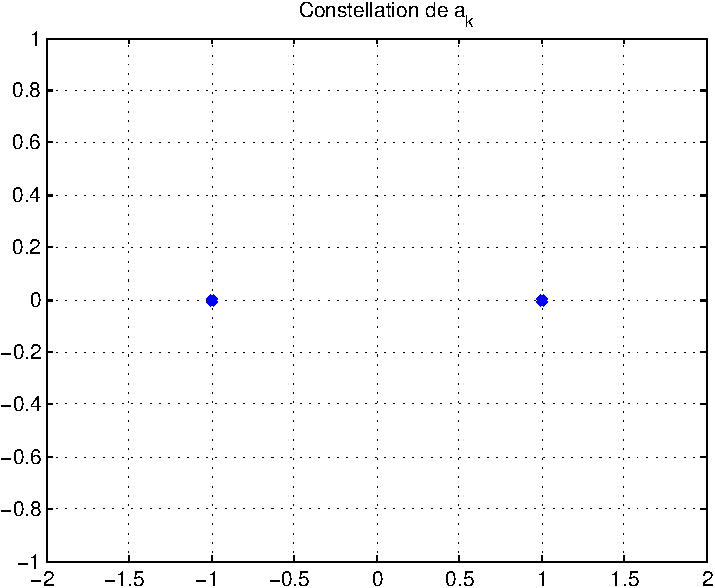
\includegraphics[scale=1]{contesllation_a_k-crop.pdf}
	\caption{Contellation des symboles $a_k$}
	\label{fig:sec1}
	\end{center}
\end{figure} 

\section{Conversion numérique - analogique}

\subsection{Expansion}
Jusqu'à maintenant les symboles sont des valeurs ponctuels dans le vecteur $a_k$. Pour "Mettre en forme" des symboles il faut les associer un signal analogique, ça n'est pas possible dans une simulateur numérique mais on peut simuler l'aspect d'un signal continu en utilisant des suréchantillonnage par symbole. Dans notre cas, le facteur de suréchantillonnage $F$ est $16$, c'est à dire que chaque symbole vas être représenté par la valeur du symbole plus $F-1=15$ zéros.

\subsubsection*{Question 1}
L'operation d'expansion est fait à la fonction \emph{expansion} et la figure \ref{fig:ques1} montre le résultat obtenu  en temps.

\begin{figure}
	\begin{center}
	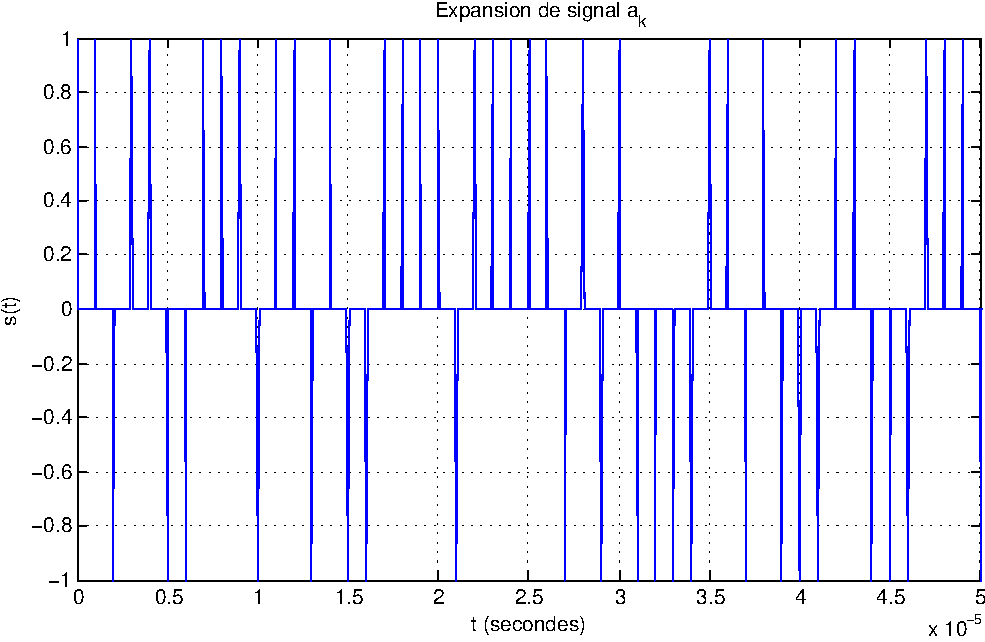
\includegraphics[scale=1]{expansion-crop.pdf}
	\caption{Expansion des symboles $a_k$}
	\label{fig:ques1}
	\end{center}
\end{figure} 

\subsection{Étude des filtres}

\subsubsection*{Question 2}
\begin{figure}
	\begin{subfigure}{.5\textwidth}
  		\centering
  		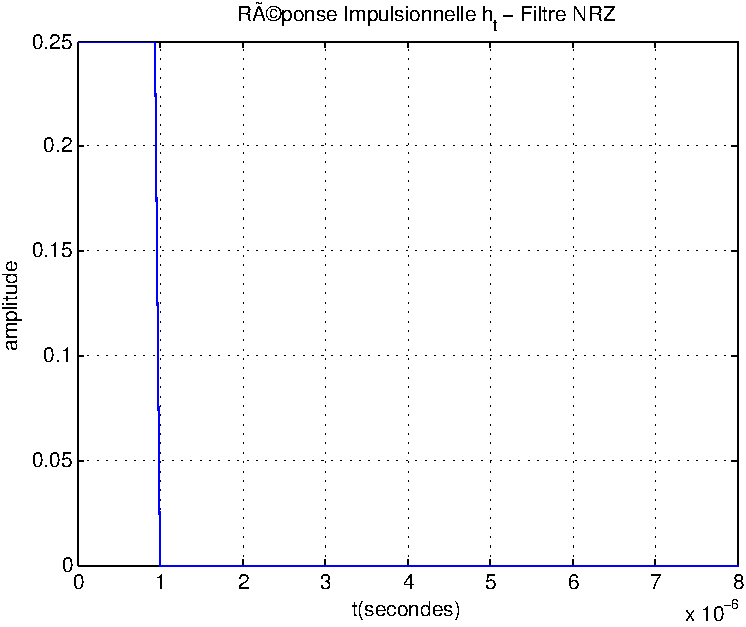
\includegraphics[width=1\linewidth]{impul_nrz-crop.pdf}
  		\caption{Réponse impulsionnelle}
  		\label{fig:nrz_impul1M}
	\end{subfigure}
	\begin{subfigure}{.5\textwidth}
  		\centering
  		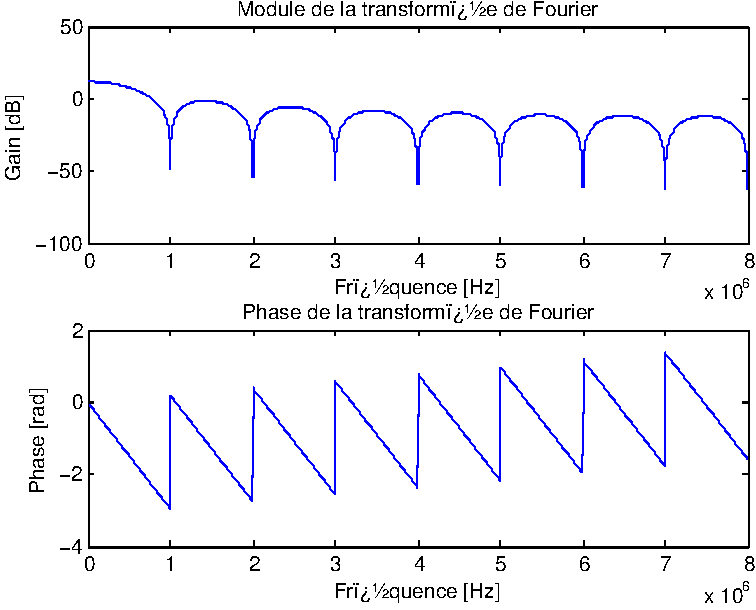
\includegraphics[width=1\linewidth]{frec_nrz-crop.pdf}
  		\caption{Réponse fréquentielle}
  		\label{fig:nrz_frec1M}
	\end{subfigure}%
	\caption{Réponse impulsionnelles et fréquentielles du filtre NRZ - $D=1 Mbit/s$}
	\label{fig:nrz1M}
\end{figure} 

\begin{figure}
	\begin{subfigure}{.5\textwidth}
  		\centering
  		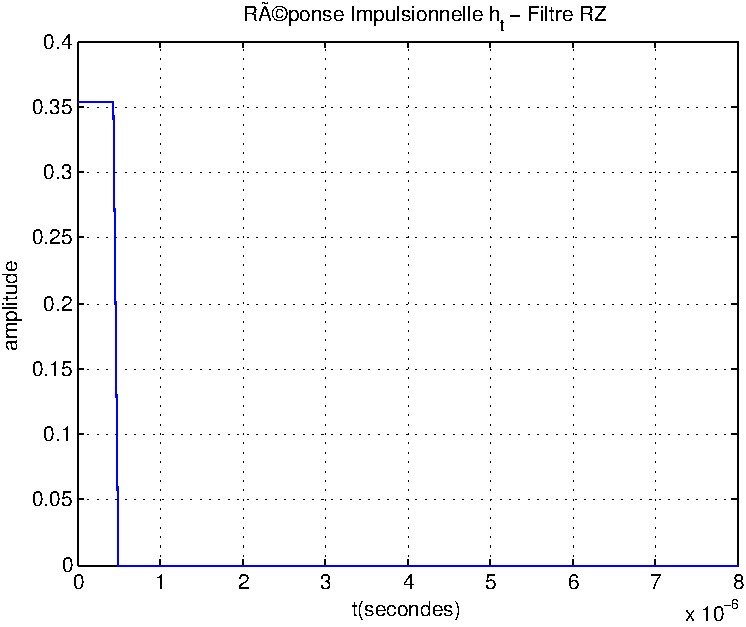
\includegraphics[width=1\linewidth]{impul_rz-crop.pdf}
  		\caption{Réponse impulsionnelle}
  		\label{fig:rz_impul1M}
	\end{subfigure}
	\begin{subfigure}{.5\textwidth}
  		\centering
  		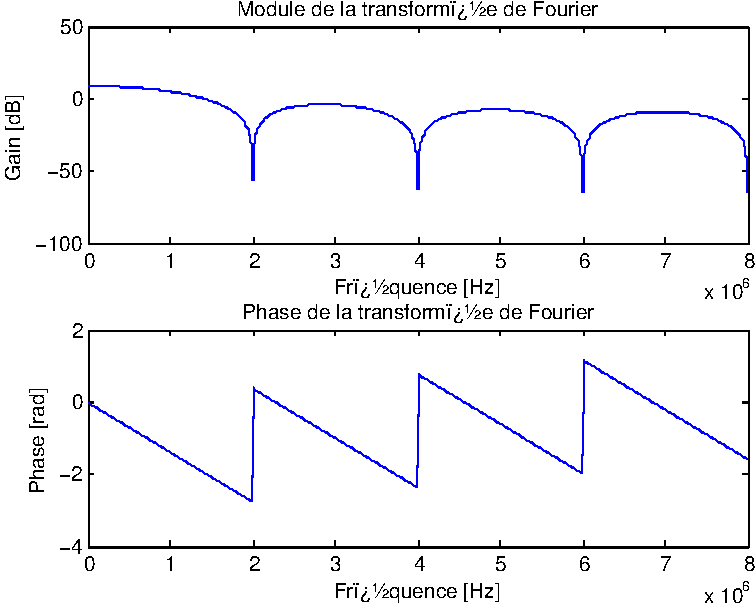
\includegraphics[width=1\linewidth]{frec_rz-crop.pdf}
  		\caption{Réponse fréquentielle}
  		\label{fig:rz_frec1M}
	\end{subfigure}%
	\caption{Réponse impulsionnelles et fréquentielles du filtre RZ - $D=1 Mbit/s$}
	\label{fig:rz1M}
\end{figure}

\begin{figure}
	\begin{subfigure}{.5\textwidth}
  		\centering
  		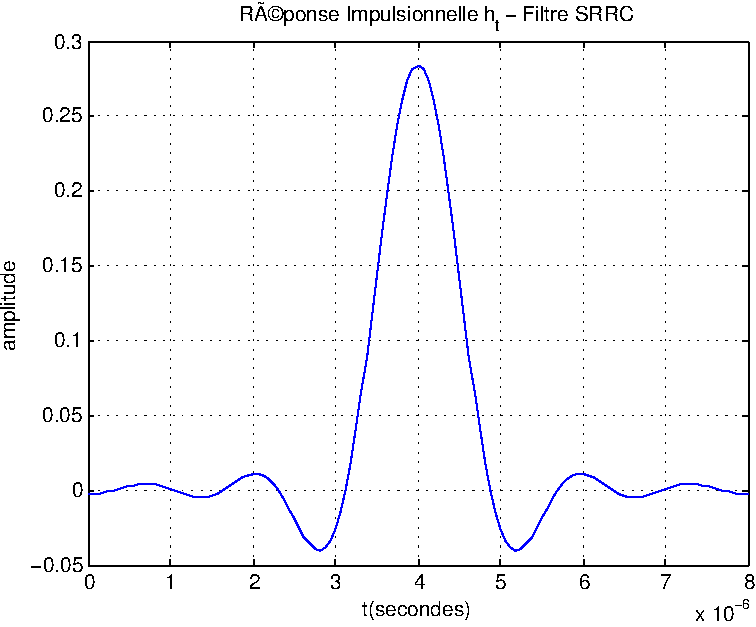
\includegraphics[width=1\linewidth]{impul_srrc-crop.pdf}
  		\caption{Réponse impulsionnelle}
  		\label{fig:srrc_impul1M}
	\end{subfigure}
	\begin{subfigure}{.5\textwidth}
  		\centering
  		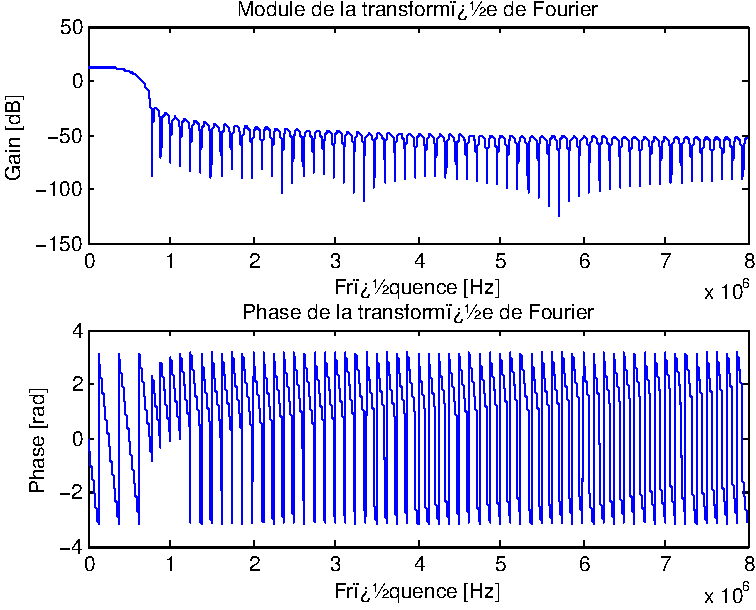
\includegraphics[width=1\linewidth]{frec_srrc-crop.pdf}
  		\caption{Réponse fréquentielle}
  		\label{fig:srrc_frec1M}
	\end{subfigure}%
	\caption{Réponse impulsionnelles et fréquentielles du filtre SRRC - $D=15 Mbit/s ; \alpha =0.5$.}
	\label{fig:srrc1M}
\end{figure} 

%------------------15Mb
\begin{figure}
	\begin{subfigure}{.5\textwidth}
  		\centering
  		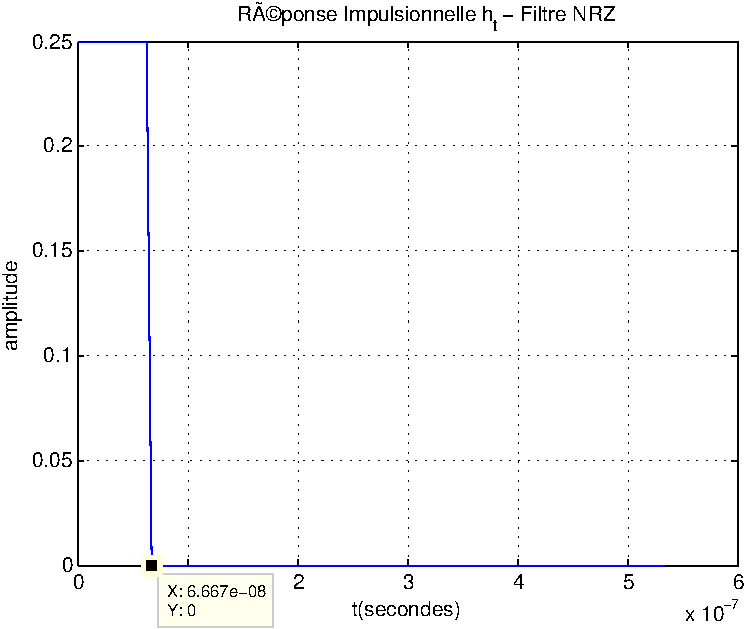
\includegraphics[width=1\linewidth]{impul_nrz_15-crop.pdf}
  		\caption{Réponse impulsionnelle}
  		\label{fig:nrz_impul15M}
	\end{subfigure}
	\begin{subfigure}{.5\textwidth}
  		\centering
  		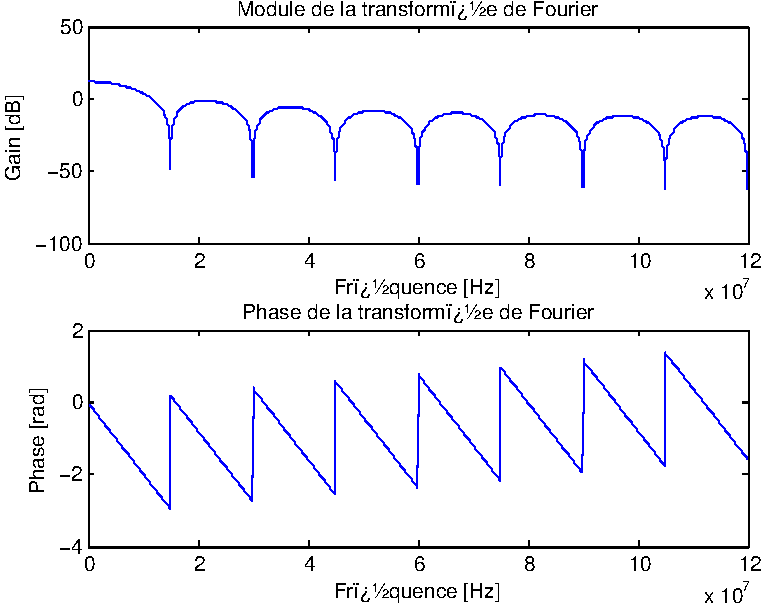
\includegraphics[width=1\linewidth]{frec_nrz_15-crop.pdf}
  		\caption{Réponse fréquentielle}
  		\label{fig:nrz_frec15M}
	\end{subfigure}%
	\caption{Réponse impulsionnelles et fréquentielles du filtre NRZ - $D=15 Mbit/s$}
	\label{fig:nrz1M}
\end{figure} 

\begin{figure}
	\begin{subfigure}{.5\textwidth}
  		\centering
  		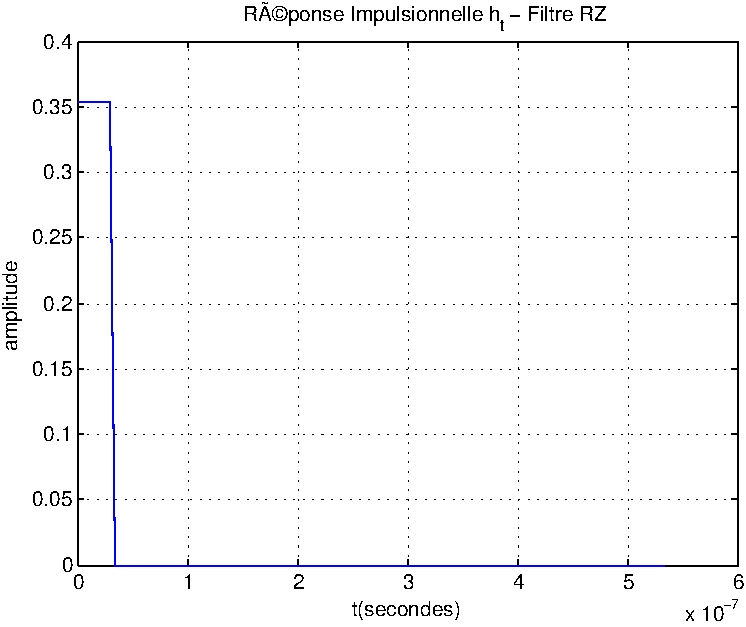
\includegraphics[width=1\linewidth]{impul_rz_15-crop.pdf}
  		\caption{Réponse impulsionnelle}
  		\label{fig:rz_impul15M}
	\end{subfigure}
	\begin{subfigure}{.5\textwidth}
  		\centering
  		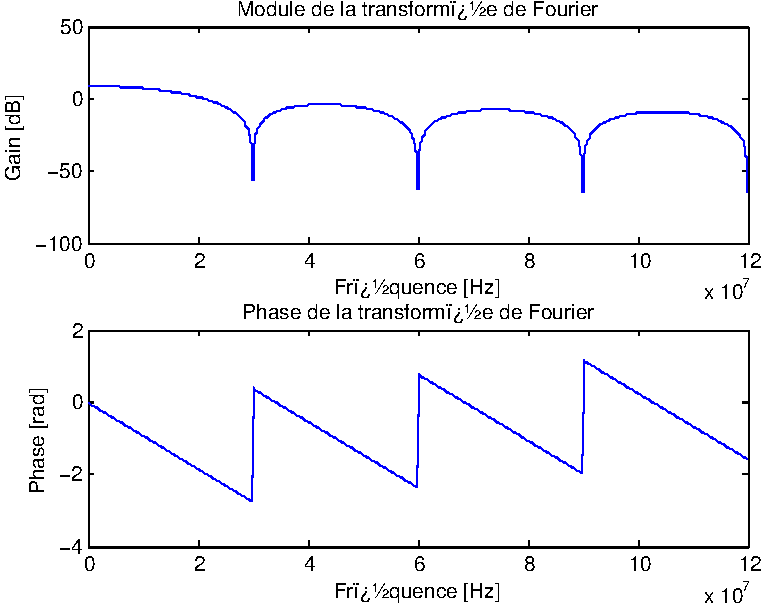
\includegraphics[width=1\linewidth]{frec_rz_15-crop.pdf}
  		\caption{Réponse fréquentielle}
  		\label{fig:rz_frec15M}
	\end{subfigure}%
	\caption{Réponse impulsionnelles et fréquentielles du filtre RZ - $D=15 Mbit/s$}
	\label{fig:rz15M}
\end{figure}

\begin{figure}
	\begin{subfigure}{.5\textwidth}
  		\centering
  		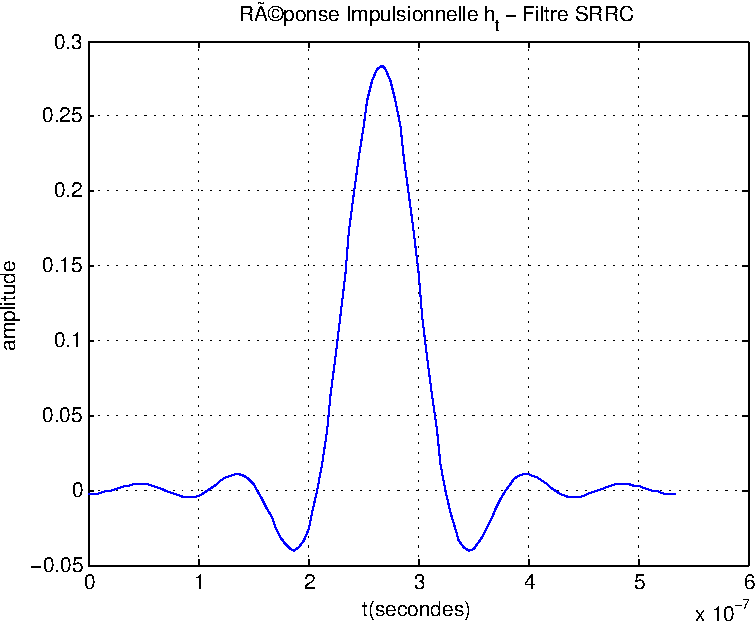
\includegraphics[width=1\linewidth]{impul_srrc_15-crop.pdf}
  		\caption{Réponse impulsionnelle}
  		\label{fig:srrc_impul15M}
	\end{subfigure}
	\begin{subfigure}{.5\textwidth}
  		\centering
  		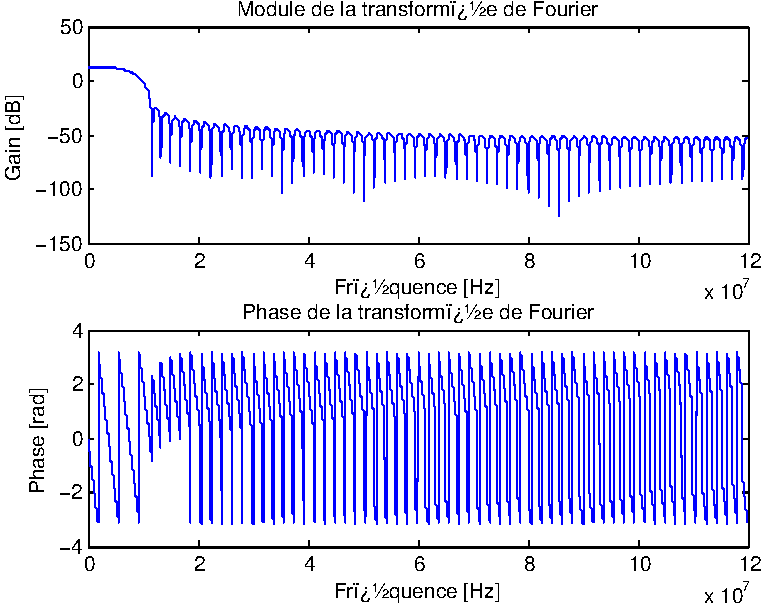
\includegraphics[width=1\linewidth]{frec_srrc_15-crop.pdf}
  		\caption{Réponse fréquentielle}
  		\label{fig:srrc_frec15M}
	\end{subfigure}%
	\caption{Réponse impulsionnelles et fréquentielles du filtre SRRC - $D=15 Mbit/s ; \alpha =0.5$.}
	\label{fig:srrc15M}
\end{figure}

%-------------------1M alpha 0
\begin{figure}[htb]
	\begin{subfigure}{.5\textwidth}
  		\centering
  		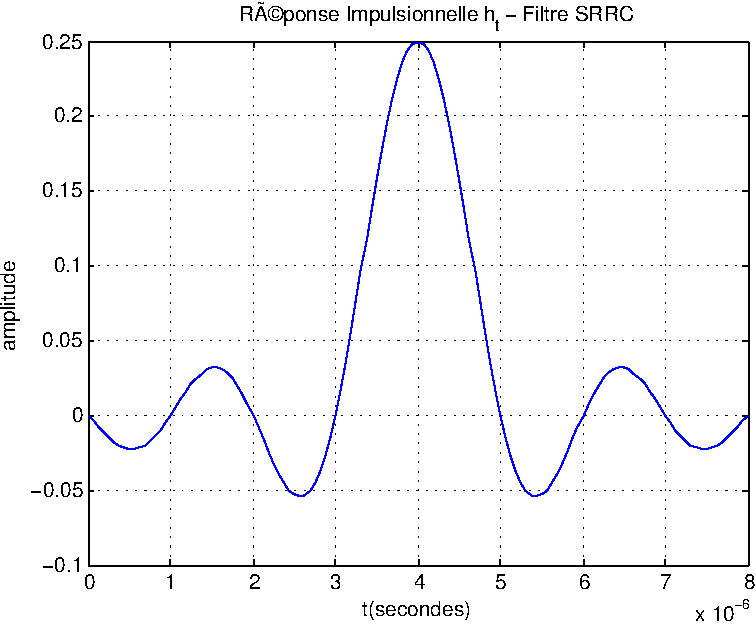
\includegraphics[width=1\linewidth]{impul_srrc_alpha_0-crop.pdf}
  		\caption{Réponse impulsionnelle}
  		\label{fig:srrc_impul15M_alp0}
	\end{subfigure}
	\begin{subfigure}{.5\textwidth}
  		\centering
  		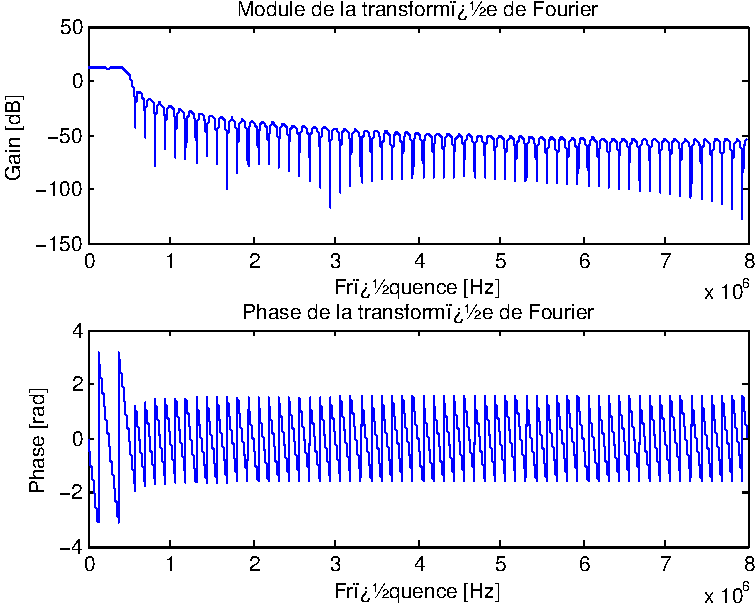
\includegraphics[width=1\linewidth]{frec_srrc_alpha_0-crop.pdf}
  		\caption{Réponse fréquentielle}
  		\label{fig:srrc_frec15M_alp0}
	\end{subfigure}%
	\caption{Réponse impulsionnelles et fréquentielles du filtre SRRC - $D=15 Mbit/s ; \alpha =0$.}
	\label{fig:srrc15M_alp0}
\end{figure}

%-------------------1M alpha 1
\begin{figure}[htb]
	\begin{subfigure}{.5\textwidth}
  		\centering
  		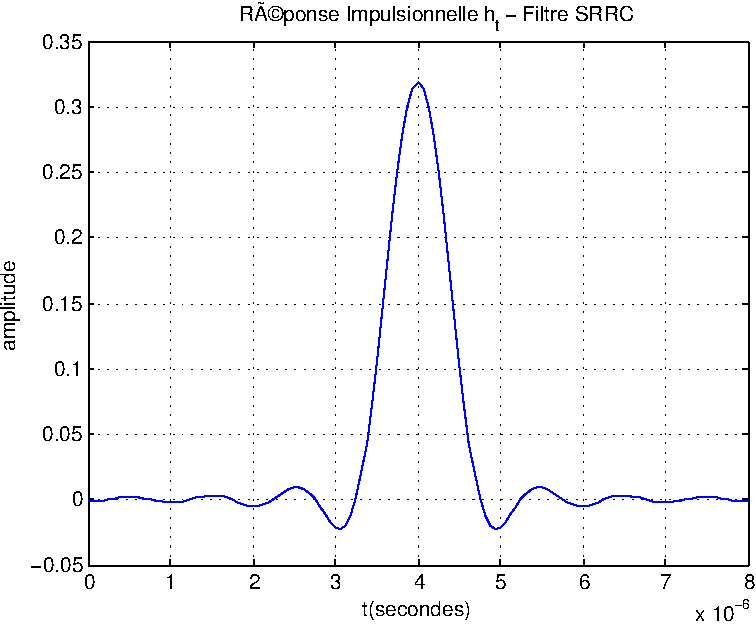
\includegraphics[width=1\linewidth]{impul_srrc_alpha_1-crop.pdf}
  		\caption{Réponse impulsionnelle}
  		\label{fig:srrc_impul15M_alp1}
	\end{subfigure}
	\begin{subfigure}{.5\textwidth}
  		\centering
  		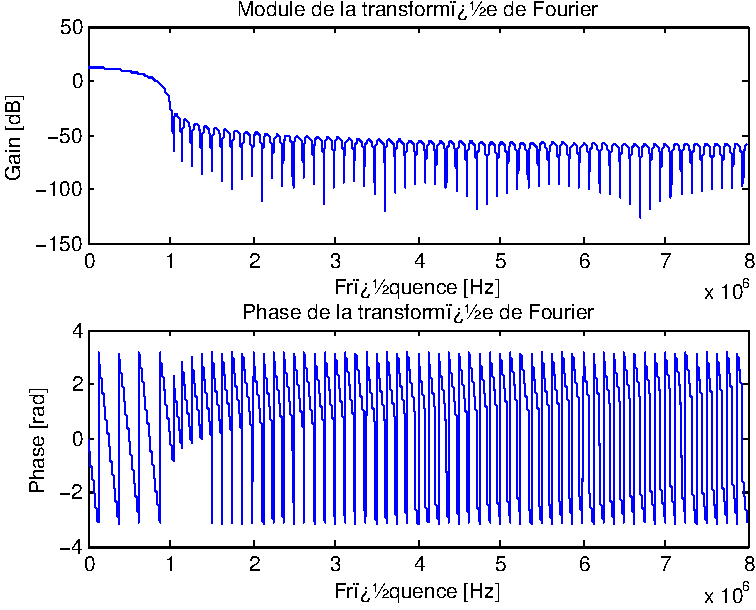
\includegraphics[width=1\linewidth]{frec_srrc_alpha_1-crop.pdf}
  		\caption{Réponse fréquentielle}
  		\label{fig:srrc_frec15M_alp1}
	\end{subfigure}%
	\caption{Réponse impulsionnelles et fréquentielles du filtre SRRC - $D=15 Mbit/s ; \alpha =1$.}
	\label{fig:srrc15M_alp1}
\end{figure}
  

\subsection{Mise en forme des symboles}

\subsubsection*{Question 3}

\begin{figure}[htb]
	\begin{center}
	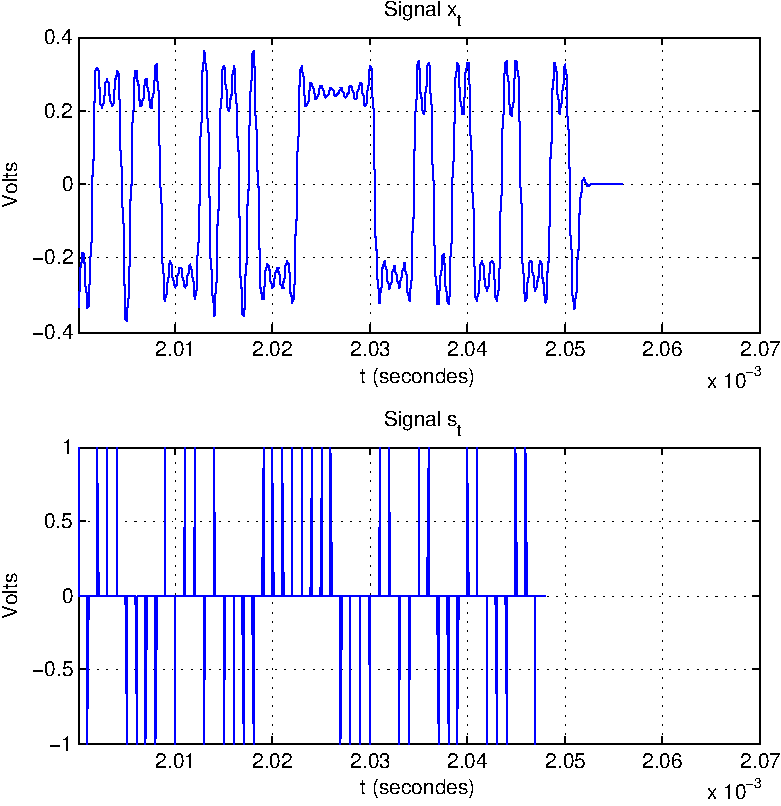
\includegraphics[scale=1]{question3-crop.pdf}
	\caption{Mise en forme des symboles $a_k$}
	\label{fig:ques3}
	\end{center}
\end{figure} 

\subsubsection*{Question 4}

\begin{figure}[htb]
	\begin{center}
	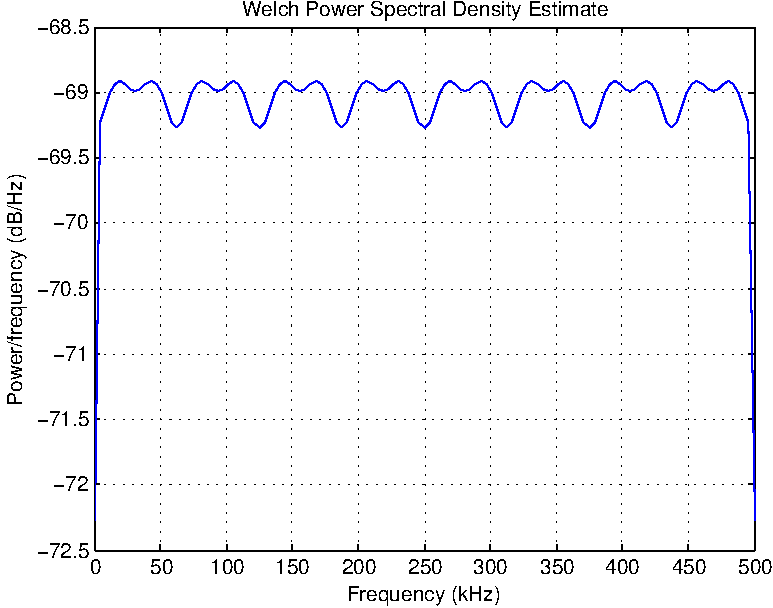
\includegraphics[scale=1]{welch_s_t-crop.pdf}
	\caption{Densité spectrale du puissance de $s_t$}
	\label{fig:ques4_st}
	\end{center}
\end{figure} 

\begin{figure}[htb]
	\begin{center}
	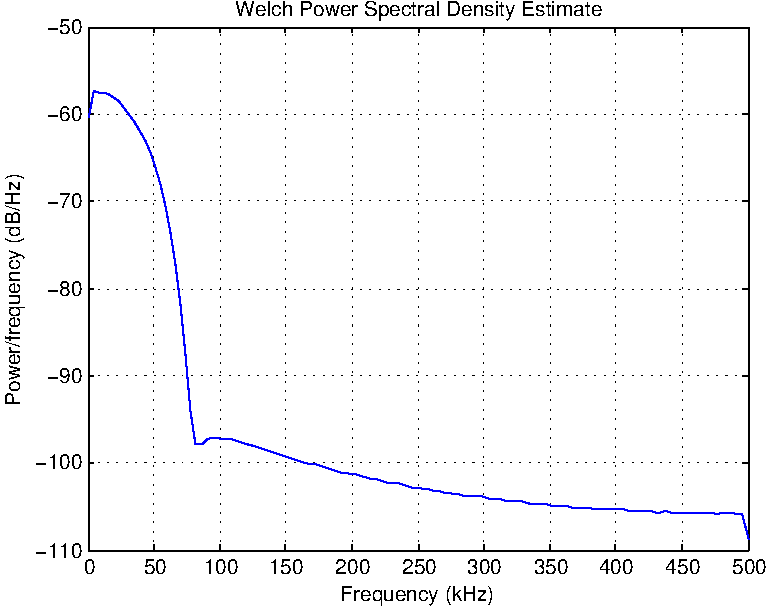
\includegraphics[scale=1]{welch_x_t-crop.pdf}
	\caption{Densité spectrale du puissance de $x_t$}
	\label{fig:ques4_xt}
	\end{center}
\end{figure} 


\subsubsection*{Question 5}

\begin{figure}[htb]
	\begin{center}
	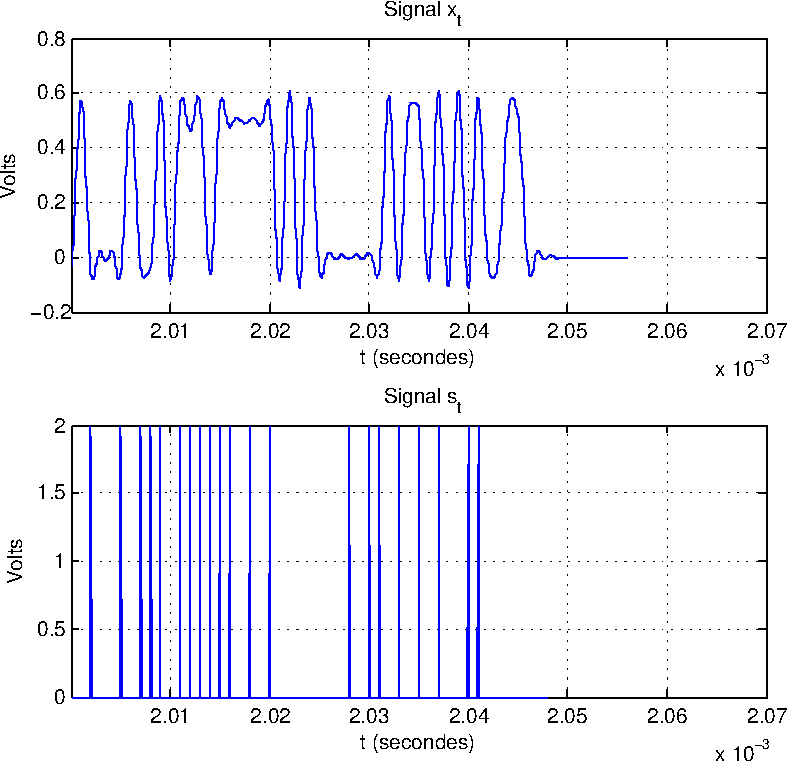
\includegraphics[scale=1]{question3_noncentree-crop.pdf}
	\caption{Mise en forme des symboles $a_k$ non-centrés.}
	\label{fig:ques5_q3}
	\end{center}
\end{figure}

\begin{figure}
	\begin{center}
	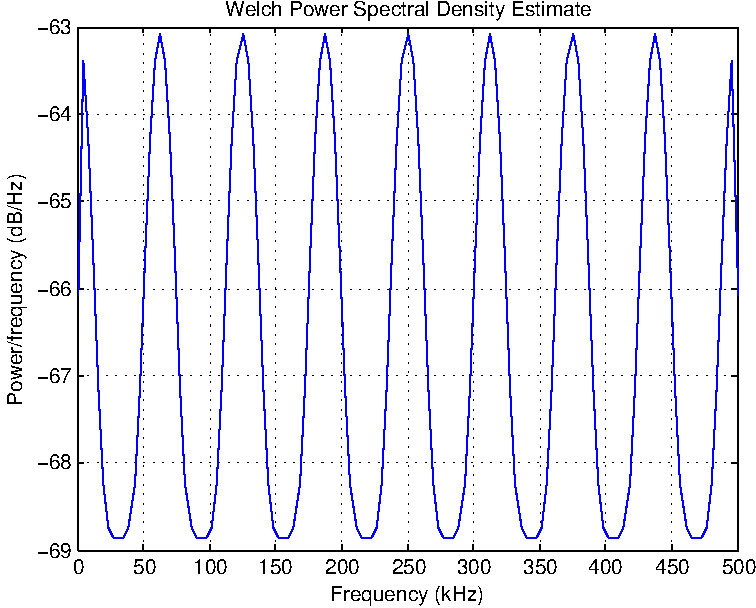
\includegraphics[scale=1]{welch_s_t_noncentree-crop.pdf}
	\caption{Densité spectrale du puissance de $s_t$ non-centrée.}
	\label{fig:ques5_Q4st}
	\end{center}
\end{figure} 

\begin{figure}
	\begin{center}
	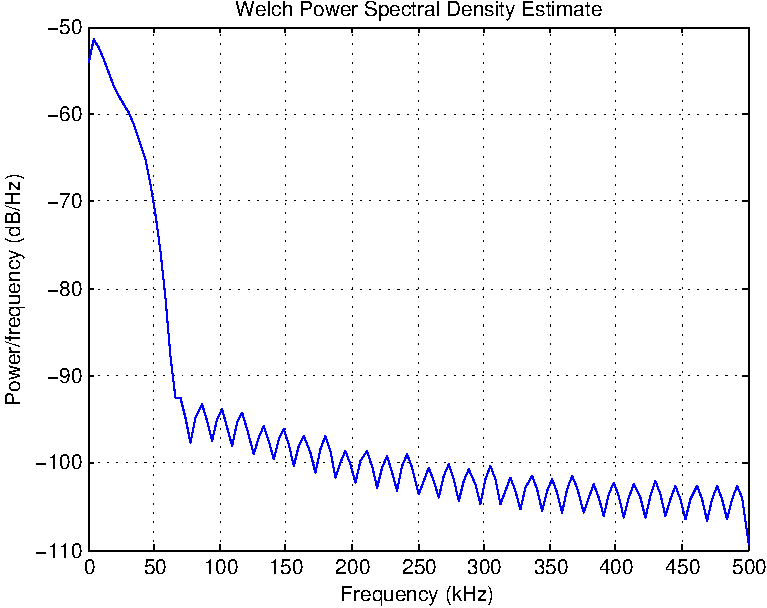
\includegraphics[scale=1]{welch_x_t_noncentree-crop.pdf}
	\caption{Densité spectrale du puissance de $x_t$ non-centrée.}
	\label{fig:ques5_Q4xt}
	\end{center}
\end{figure}

\section{Ajout du bruit blanc gaussien}
L'ajoute du bruit blanc gaussien dans un canal est inévitable. C'est pour cela que le paramètre RSB est très important et aide à mesurer la puissance du bruit dans le canal. Cette expression est:
\[ \frac{E_b}{N_0}=F\frac{\sigma ^{2}_x}{\sigma ^{2}_n}\]
Où, \[ \sigma ^{2}_n = F.N_0/T\]
\subsubsection*{Question 6}
Selon les notes du cours la formule de puissance et l'énergie de bit pour les symboles non-corrélés et centrés est:
\[ P_x=\sigma _x ^2.Ts\left \| h_e \right \|^2 \]
\[E_b=\sigma _x ^2.Ts\left \| h_e \right \|^2.T_b\]

Où, \[Ts\left \| h_e \right \|^2 = 1\]
Pour à la fin obtenir que,
\[E_b=\sigma _x ^2.T_b \]
Finalement, à partir du RSB on obtient la formule suivante:
\[\frac{E_b}{N_0}=\frac{\sigma _x ^2.T_b}{N_0} = \frac{F.\sigma _x ^2}{F.N_0/T} = 
F\frac{\sigma ^{2}_x}{\sigma ^{2}_n}
\]
Alors la valeur de la variance du signal \emph{s(t)} est:
\[\sigma _x ^2=E[a_k^2]-m_a^2= \frac{1}{2}(1^2)+\frac{1}{2}(1^2)-0=\frac{1}{4}\]
Pour cela, l'expression de la variance du bruit est:
\[\sigma _n ^2=F\frac{\sigma _x ^2}{(E_b/N_0)_{dB}}\]
\section{Conversion analogique - numérique}
Dans une chaîne de transmission, au récepteur arrive un signal bruité et des fois attenué. C'est pour cela que ce signal à besoin d'un certain traitement pour la convertir à numérique.

\subsection{Filtrage adapté}
\subsubsection*{Question 7}
Le filtre adapté est le filtre utilisé pour détecter un signal connu dans la présence de BBG. Son but est de maximiser la RSB en diminuant l'effet du bruit. En même temps le filtre adapté est aussi utile pour éliminer l'IES.
\subsubsection*{Question 8}
La forme du filtre adapté est la version inversé et decalé du filtre de mise en forme. C'est comme cela car on à besoin de maximiser la RSB. Cela a été fait via la commande \emph{fliplr}.
\begin{figure}
	\begin{center}
	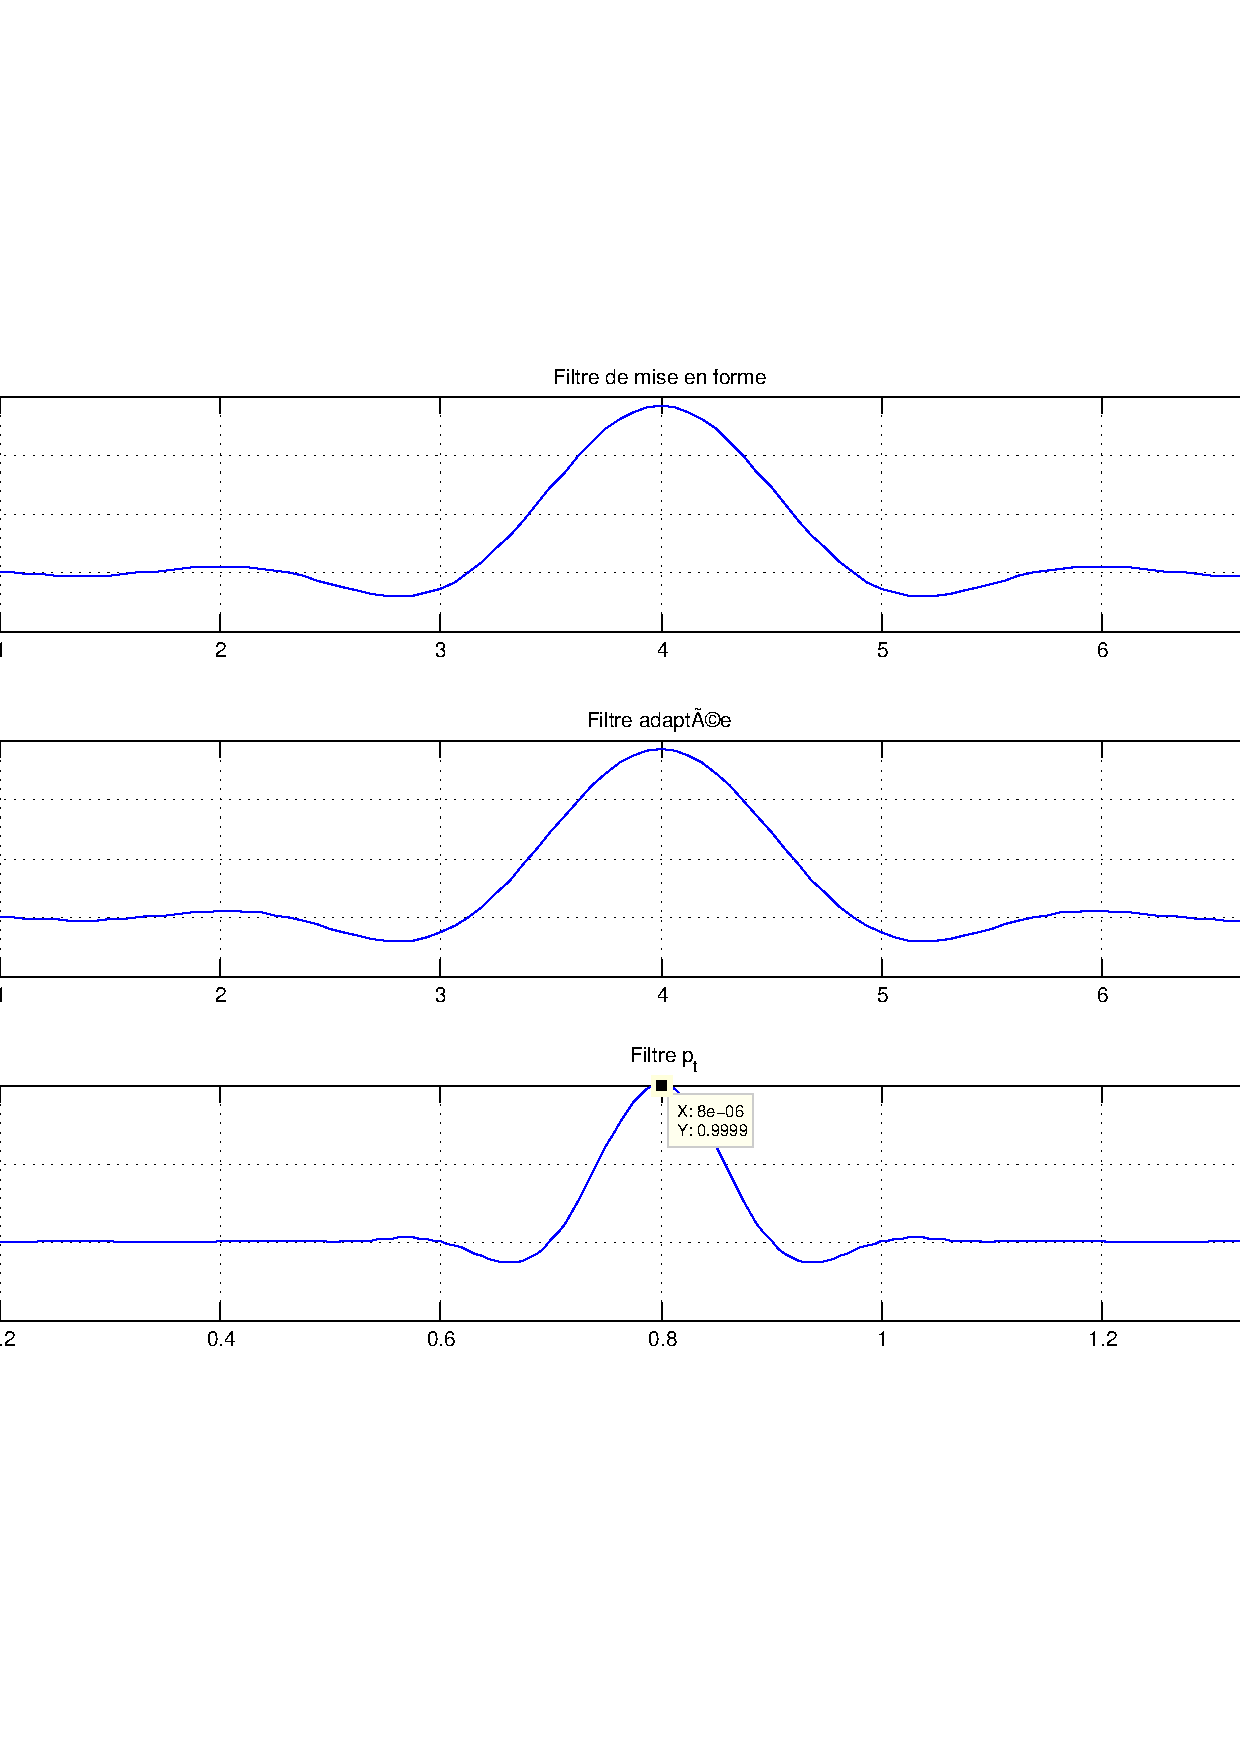
\includegraphics[scale=0.5]{Q8-1.pdf}
	\caption{Filtres de mise en forme et adapté}
	\label{fig:ques8-1}
	\end{center}
\end{figure} 
\begin{figure}
	\begin{center}
	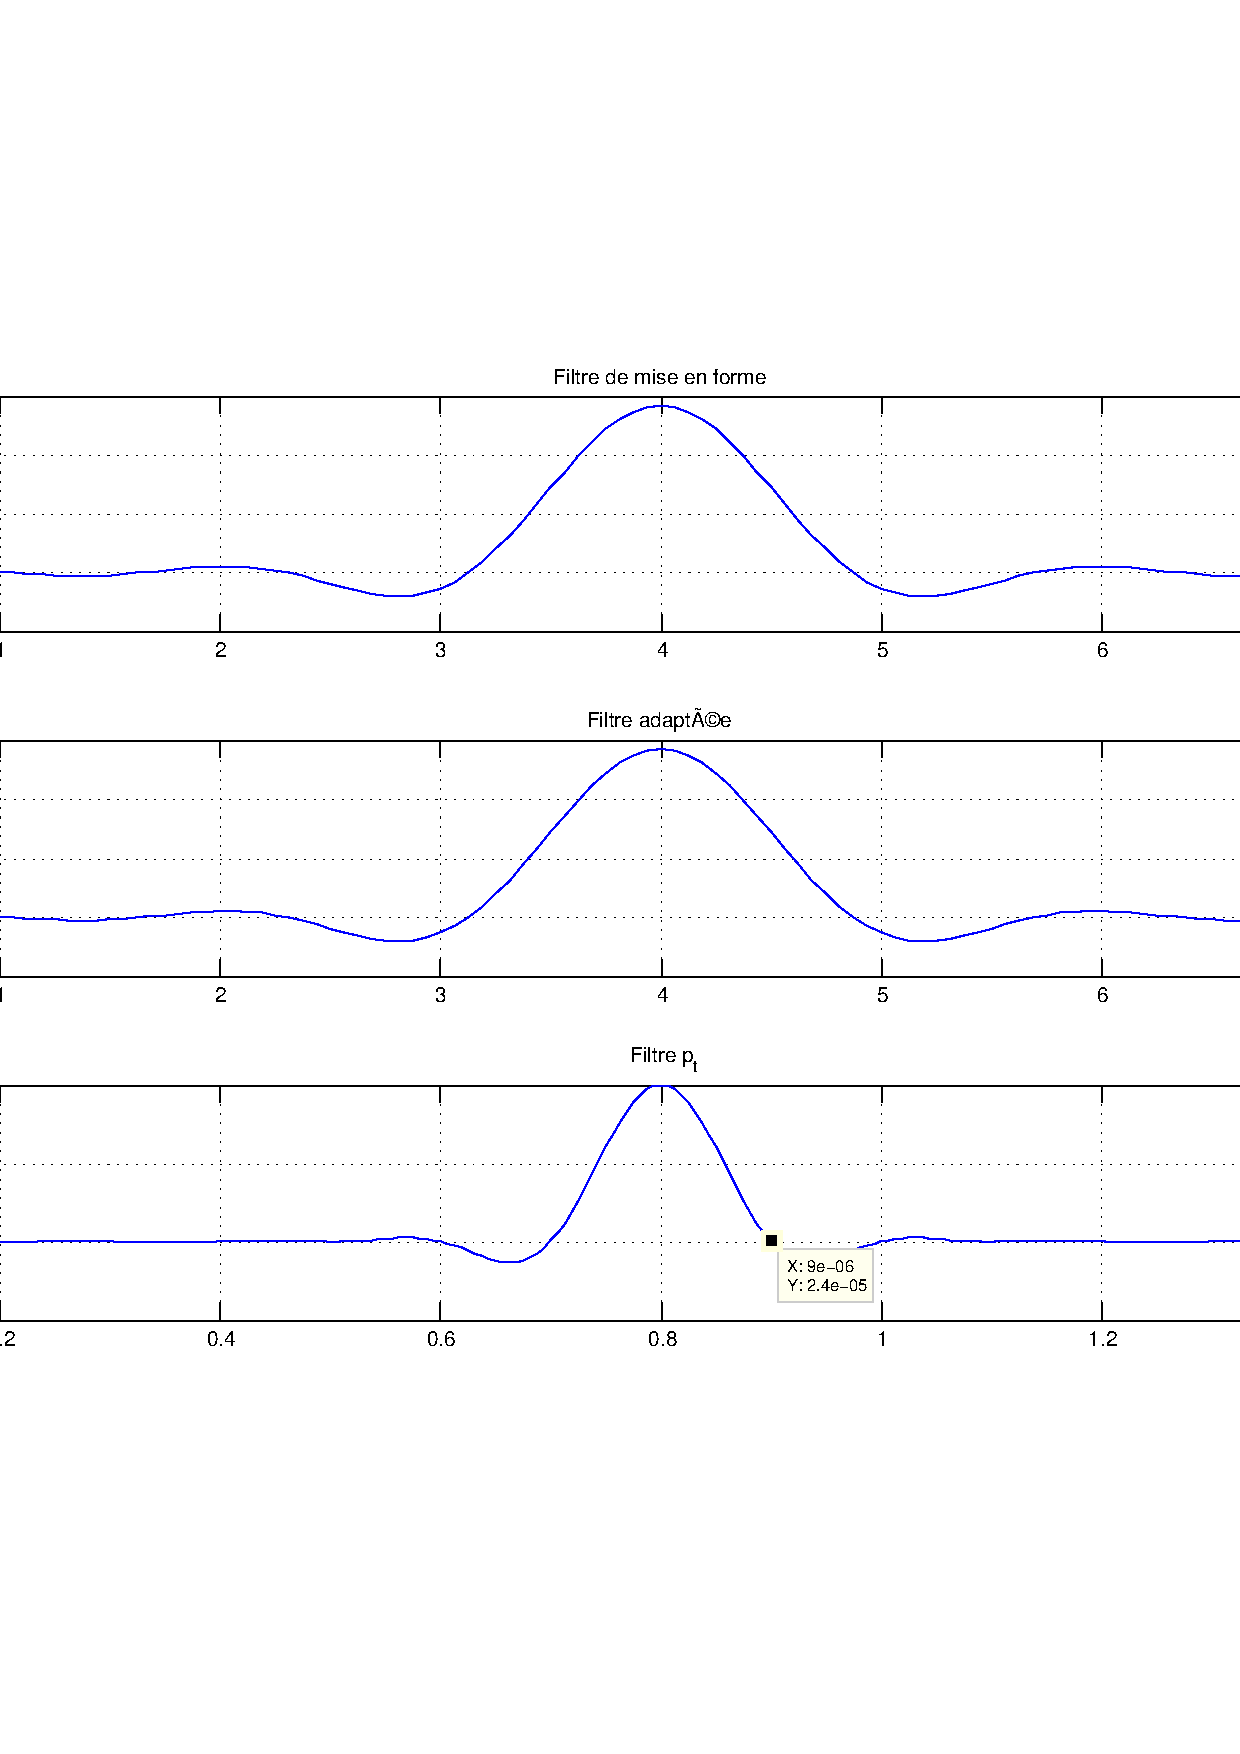
\includegraphics[scale=0.5]{Q8-2.pdf}
	\caption{Filtres de mise en forme et adapté}
	\label{fig:ques8-2}
	\end{center}
\end{figure} 
\begin{figure}
	\begin{center}
	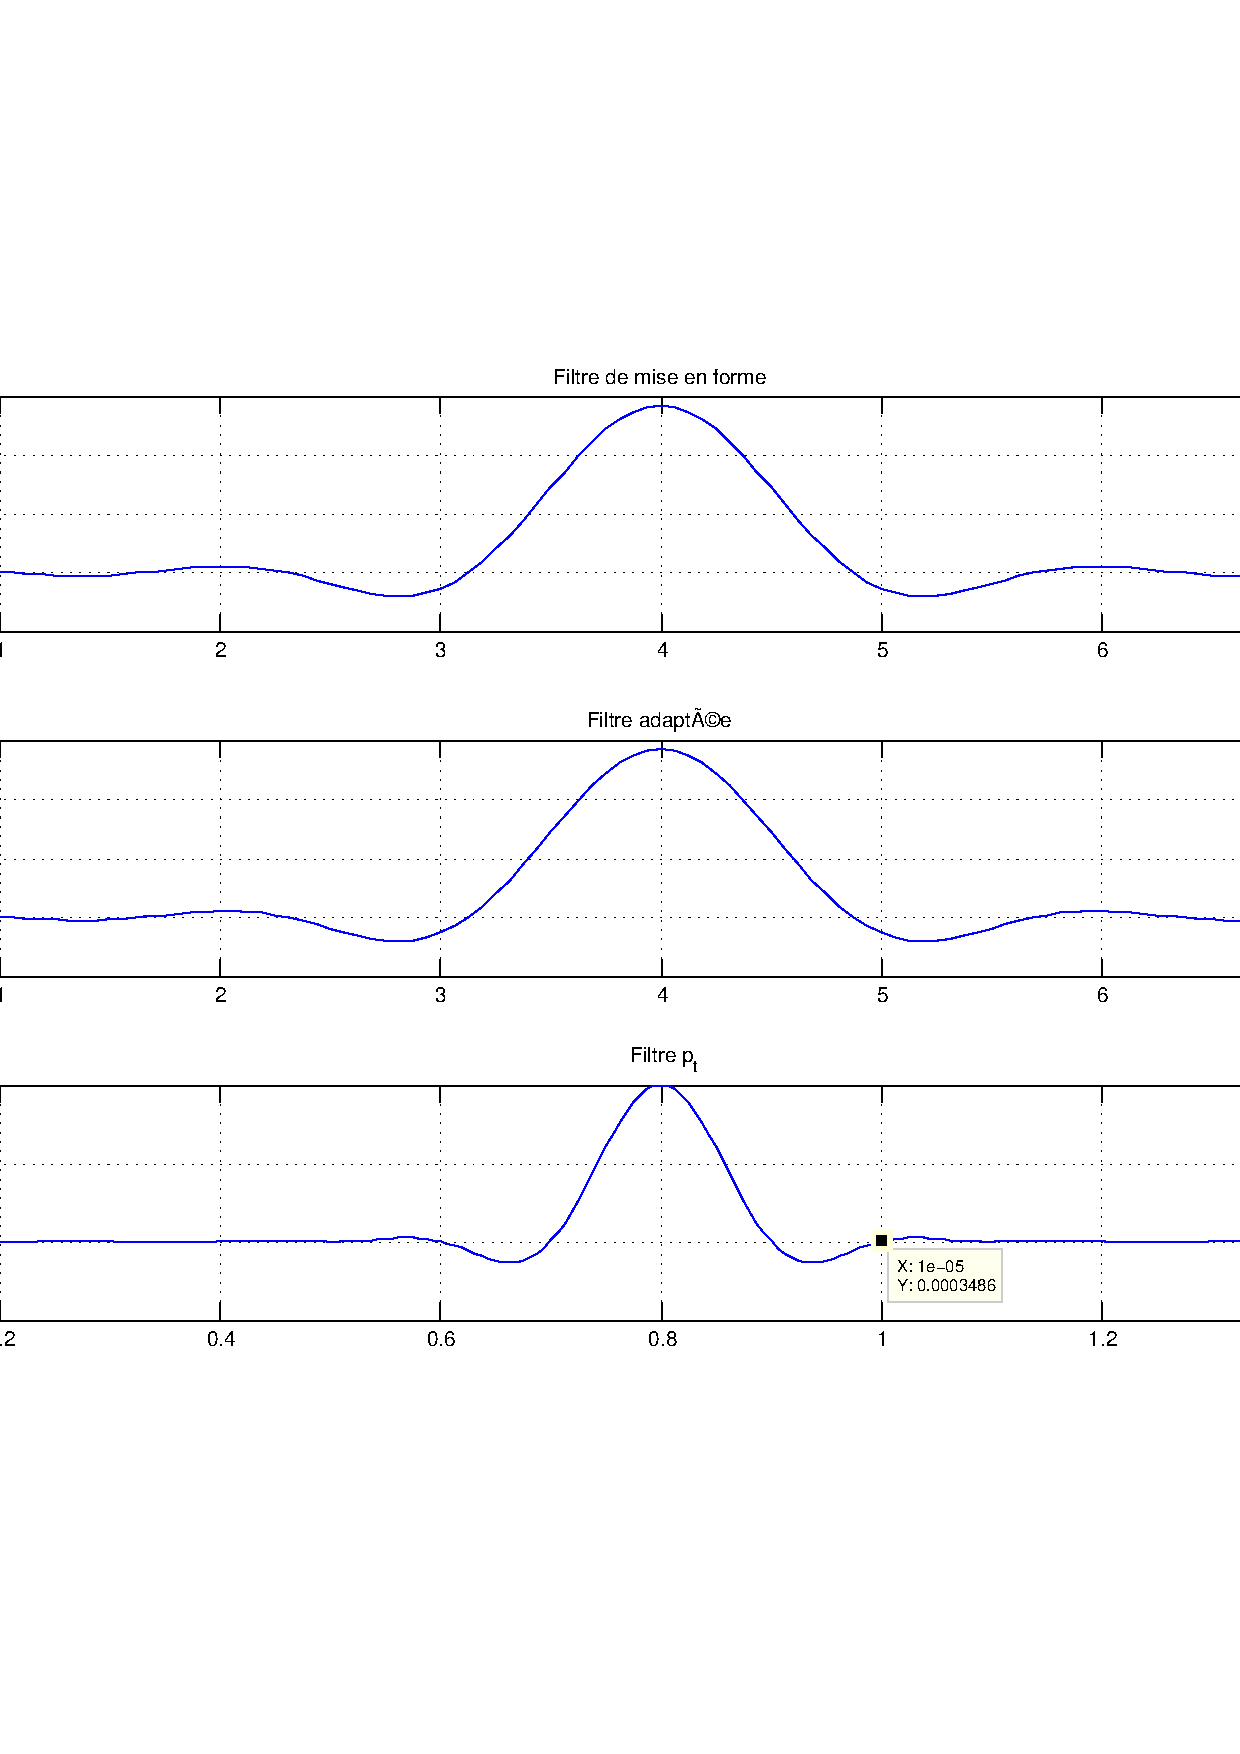
\includegraphics[scale=0.5]{Q8-3.pdf}
	\caption{Filtres de mise en forme et adapté}
	\label{fig:ques8-3}
	\end{center}
\end{figure} 


\subsubsection*{Question 9}
Comme on peut regarder dans les figures \ref{fig:ques8-1}, \ref{fig:ques8-2} et \ref{fig:ques8-3}, la sortie du filtre adapté est maximum dans le temps de bit et nul dans les multiples de ce temps, c'est pour cela qu'on vérifie qu'on peut transmettre sans IES.

\subsubsection*{Question 10}
Comme on peut regarder dans la figure \ref{fig:q10E}, c'est évident l'effet du bruit dans le diagramme de l'oeil, si on augmente la \emph{RSB} l'oeil sera plus ouvert. Pour la figure \ref{fig:q10a} on peut regarder que le diagramme change de façon que si on augmente le $\alpha$, l'oeil sera plus ouvert. Dans la figure \ref{fig:q10l} on observe que le paramètre \emph{L} n'affecte pas trop le diagramme de l'oeil. Finalement, dans la figure \ref{fig:q10t} l'effet du paramètre \emph{T} fait que les temps de symboles (où se trouve le maximum d'un symbole) soient décales.
\begin{figure}
	\begin{subfigure}{.5\textwidth}
  		\centering
  		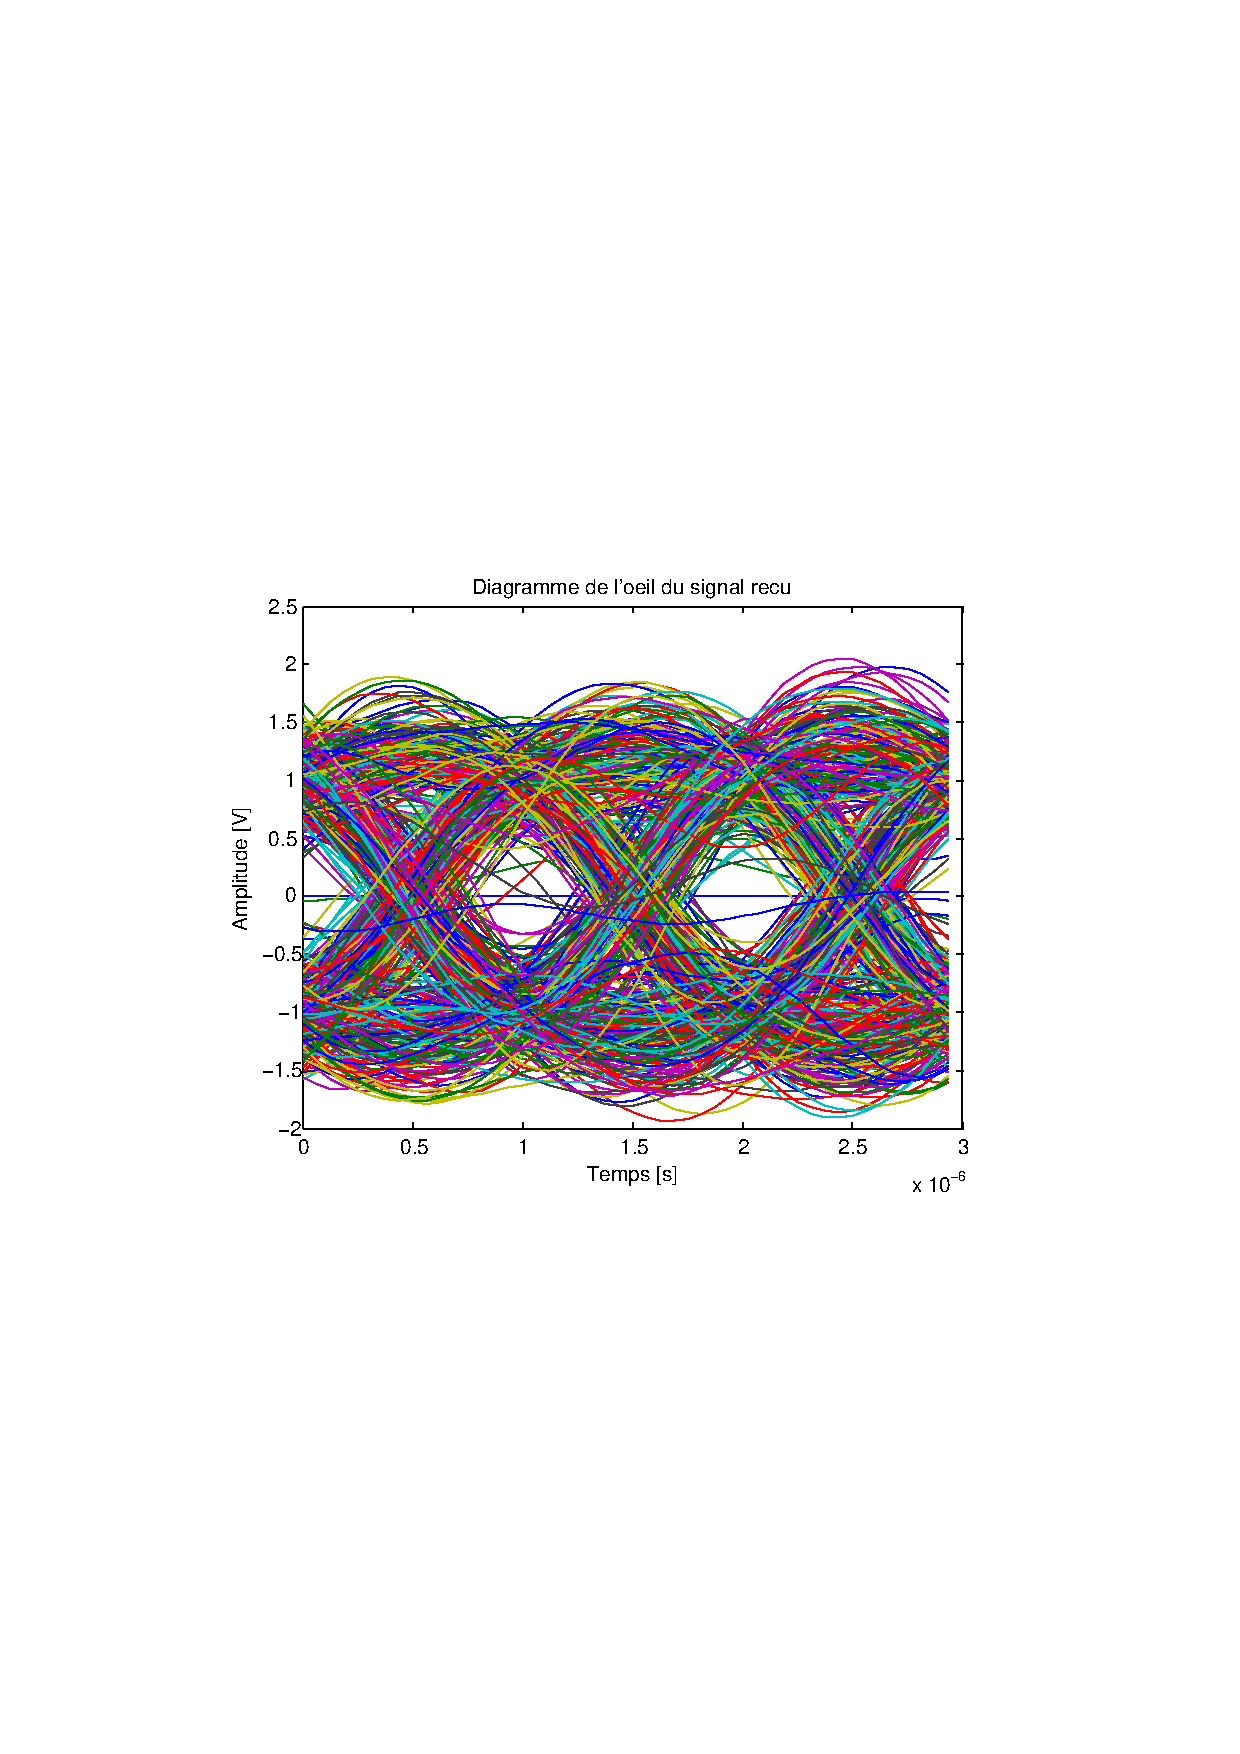
\includegraphics[width=1\linewidth]{Q10-EbNo10.pdf}
  		\caption{Diagramme de l'oeil pour RSB 10dB}
  		\label{fig:q10E10}
	\end{subfigure}
	\begin{subfigure}{.5\textwidth}
  		\centering
  		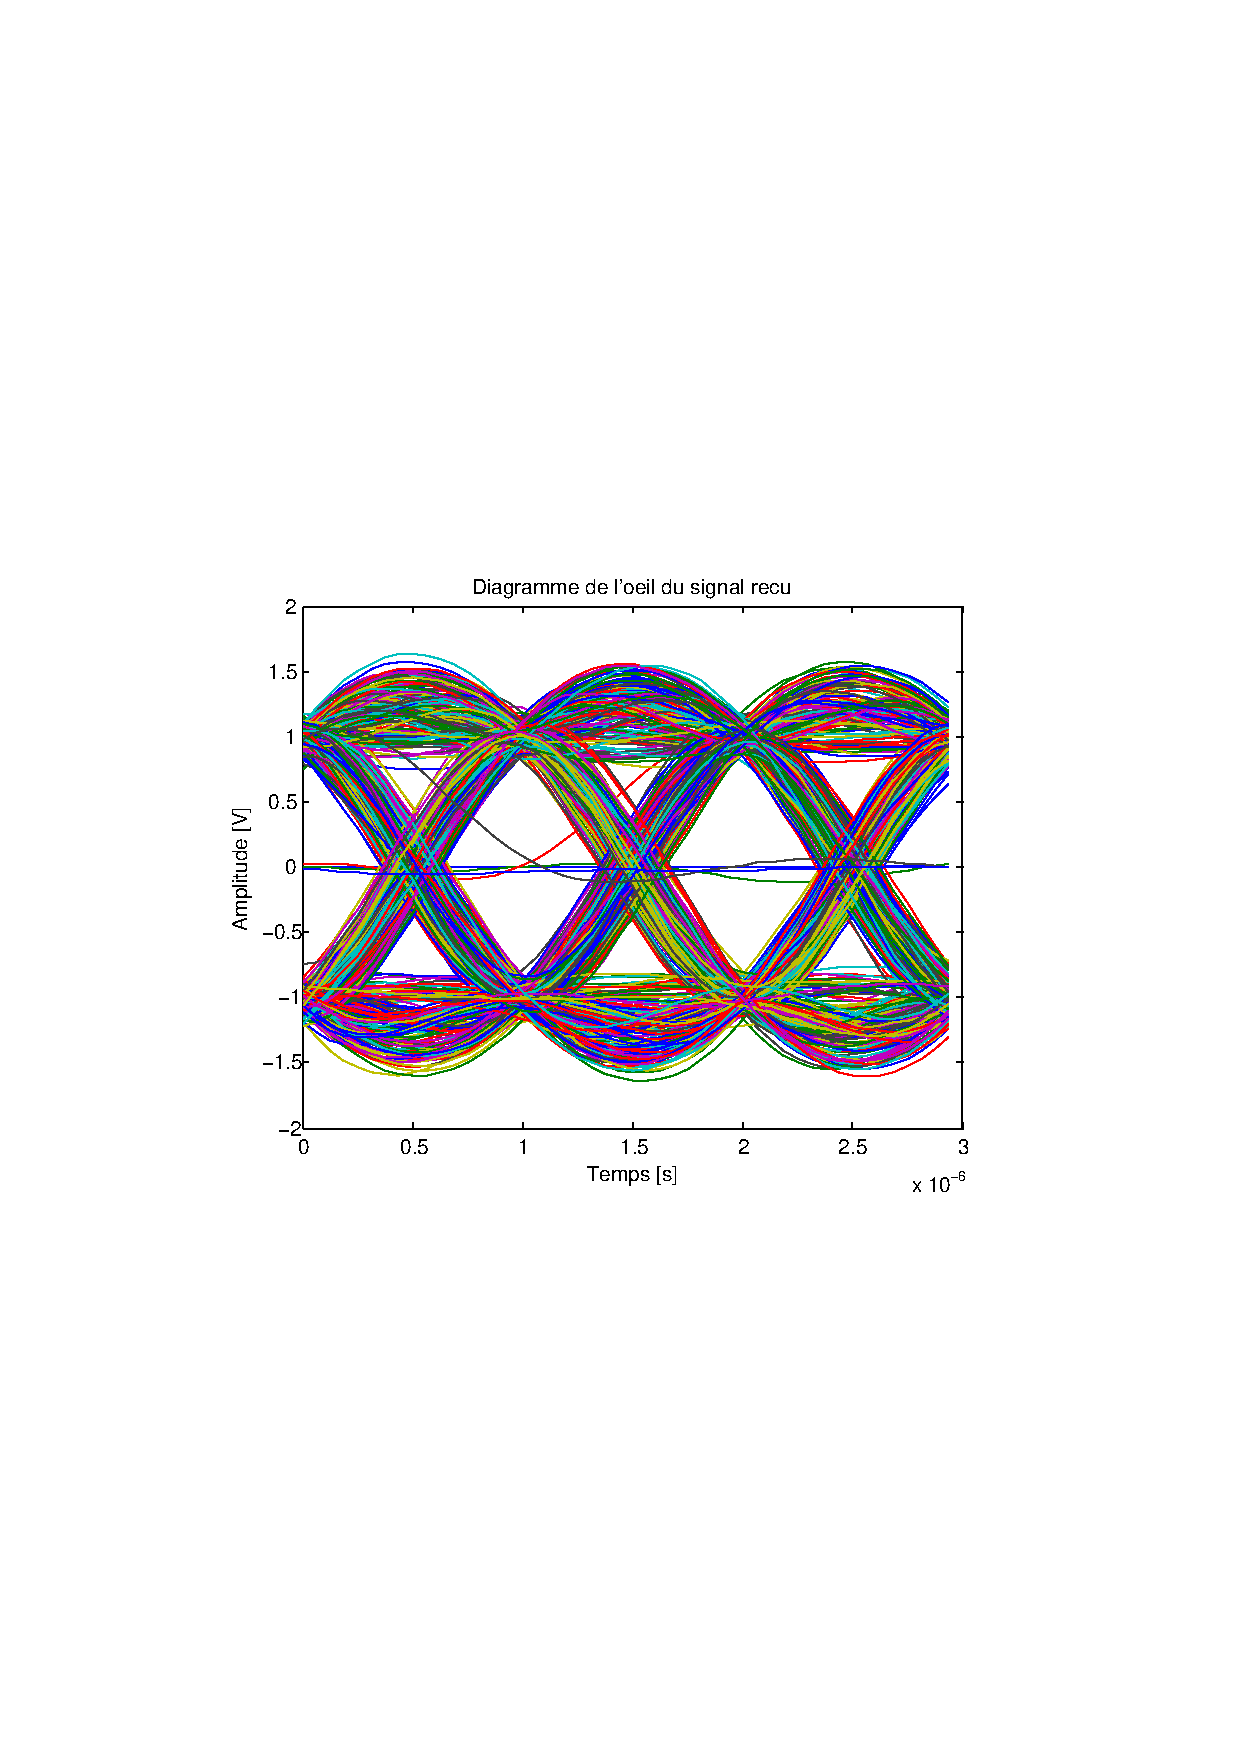
\includegraphics[width=1\linewidth]{Q10-EbNo20.pdf}
  		\caption{Diagramme de l'oeil pour RSB 20dB}
  		\label{fig:q10E20}
	\end{subfigure}
		%
	\caption{Différentes diagrammes de l'oeil à différentes \emph{RSB}.}
	\label{fig:q10E}
\end{figure}

\begin{figure}
	\begin{subfigure}{.5\textwidth}
  		\centering
  		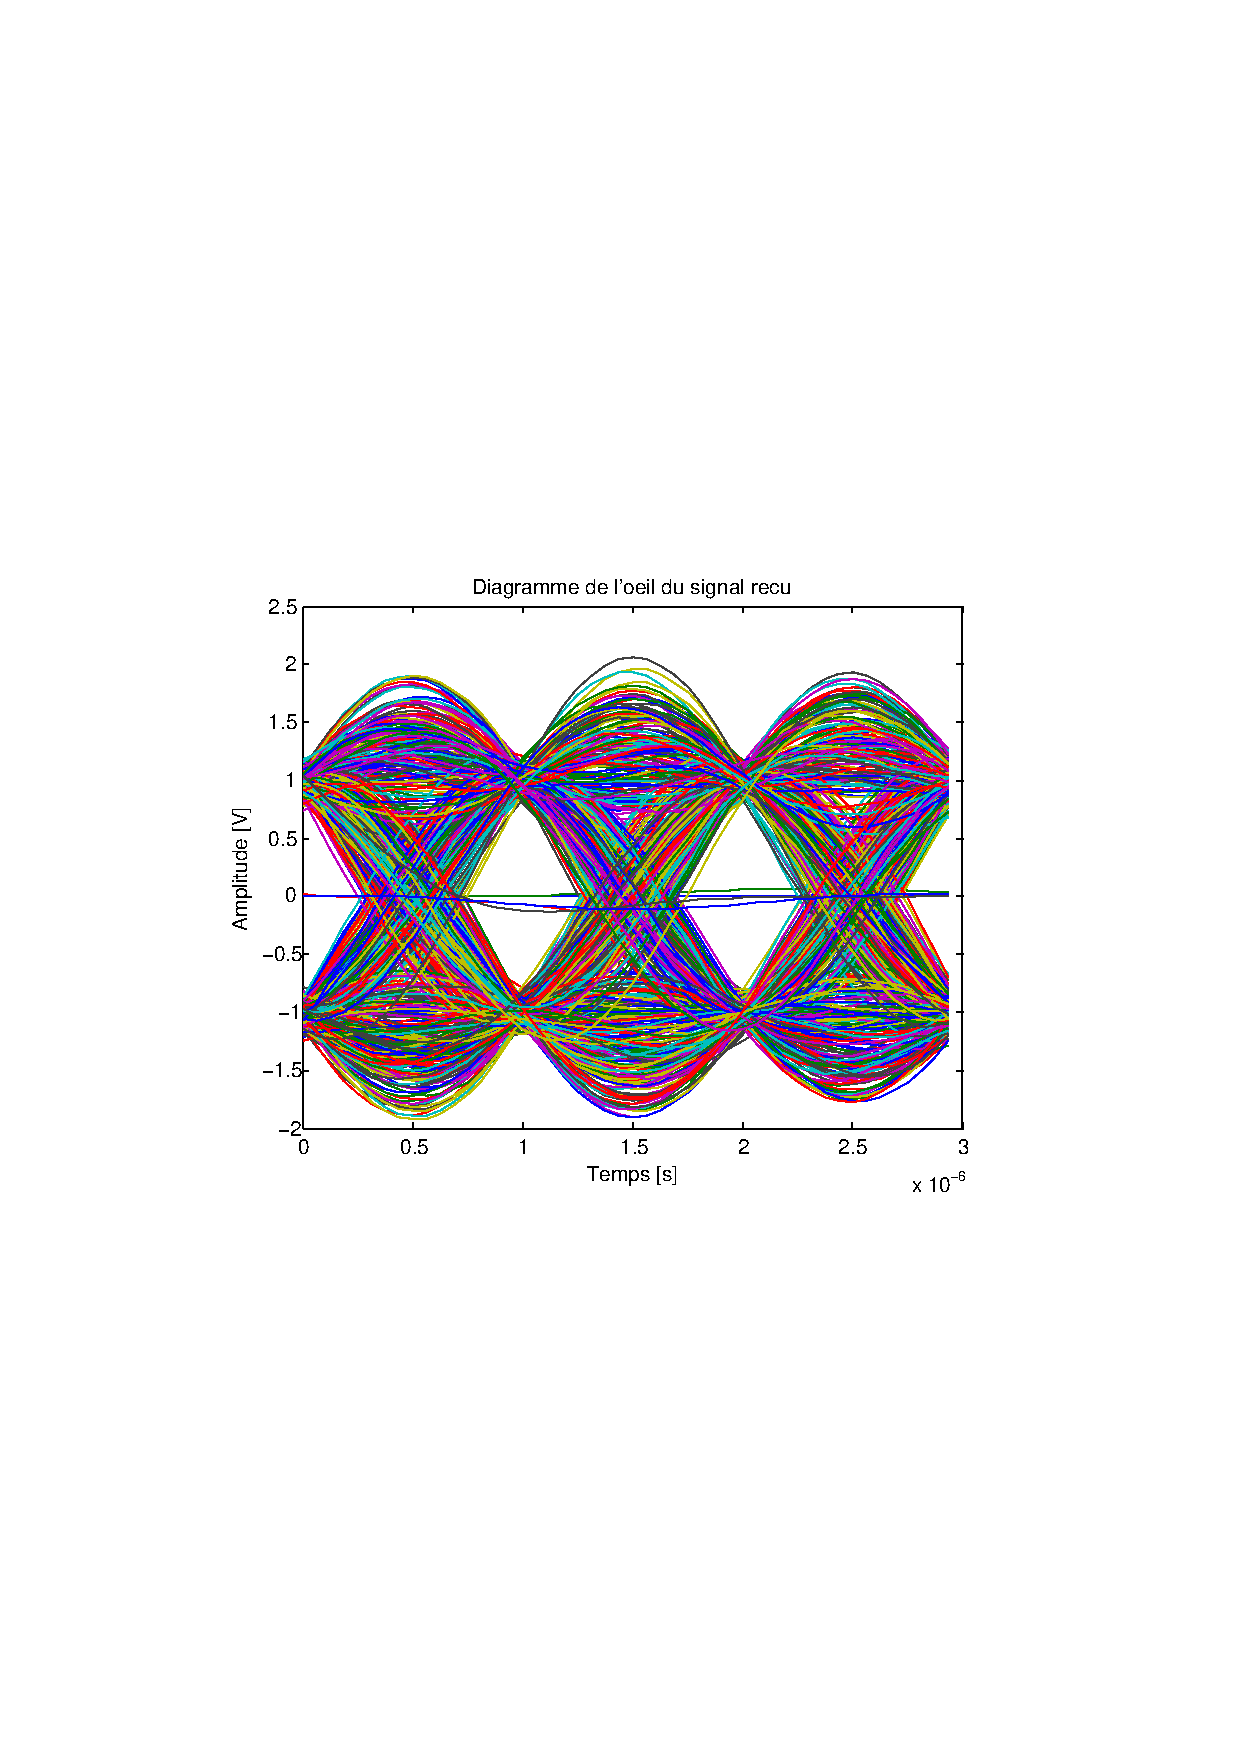
\includegraphics[width=1\linewidth]{Q10-alfa025.pdf}
  		\caption{Diagramme de l'oeil pour $\alpha$ = 0.25}
  		\label{fig:q10a025}
	\end{subfigure}
	\begin{subfigure}{.5\textwidth}
  		\centering
  		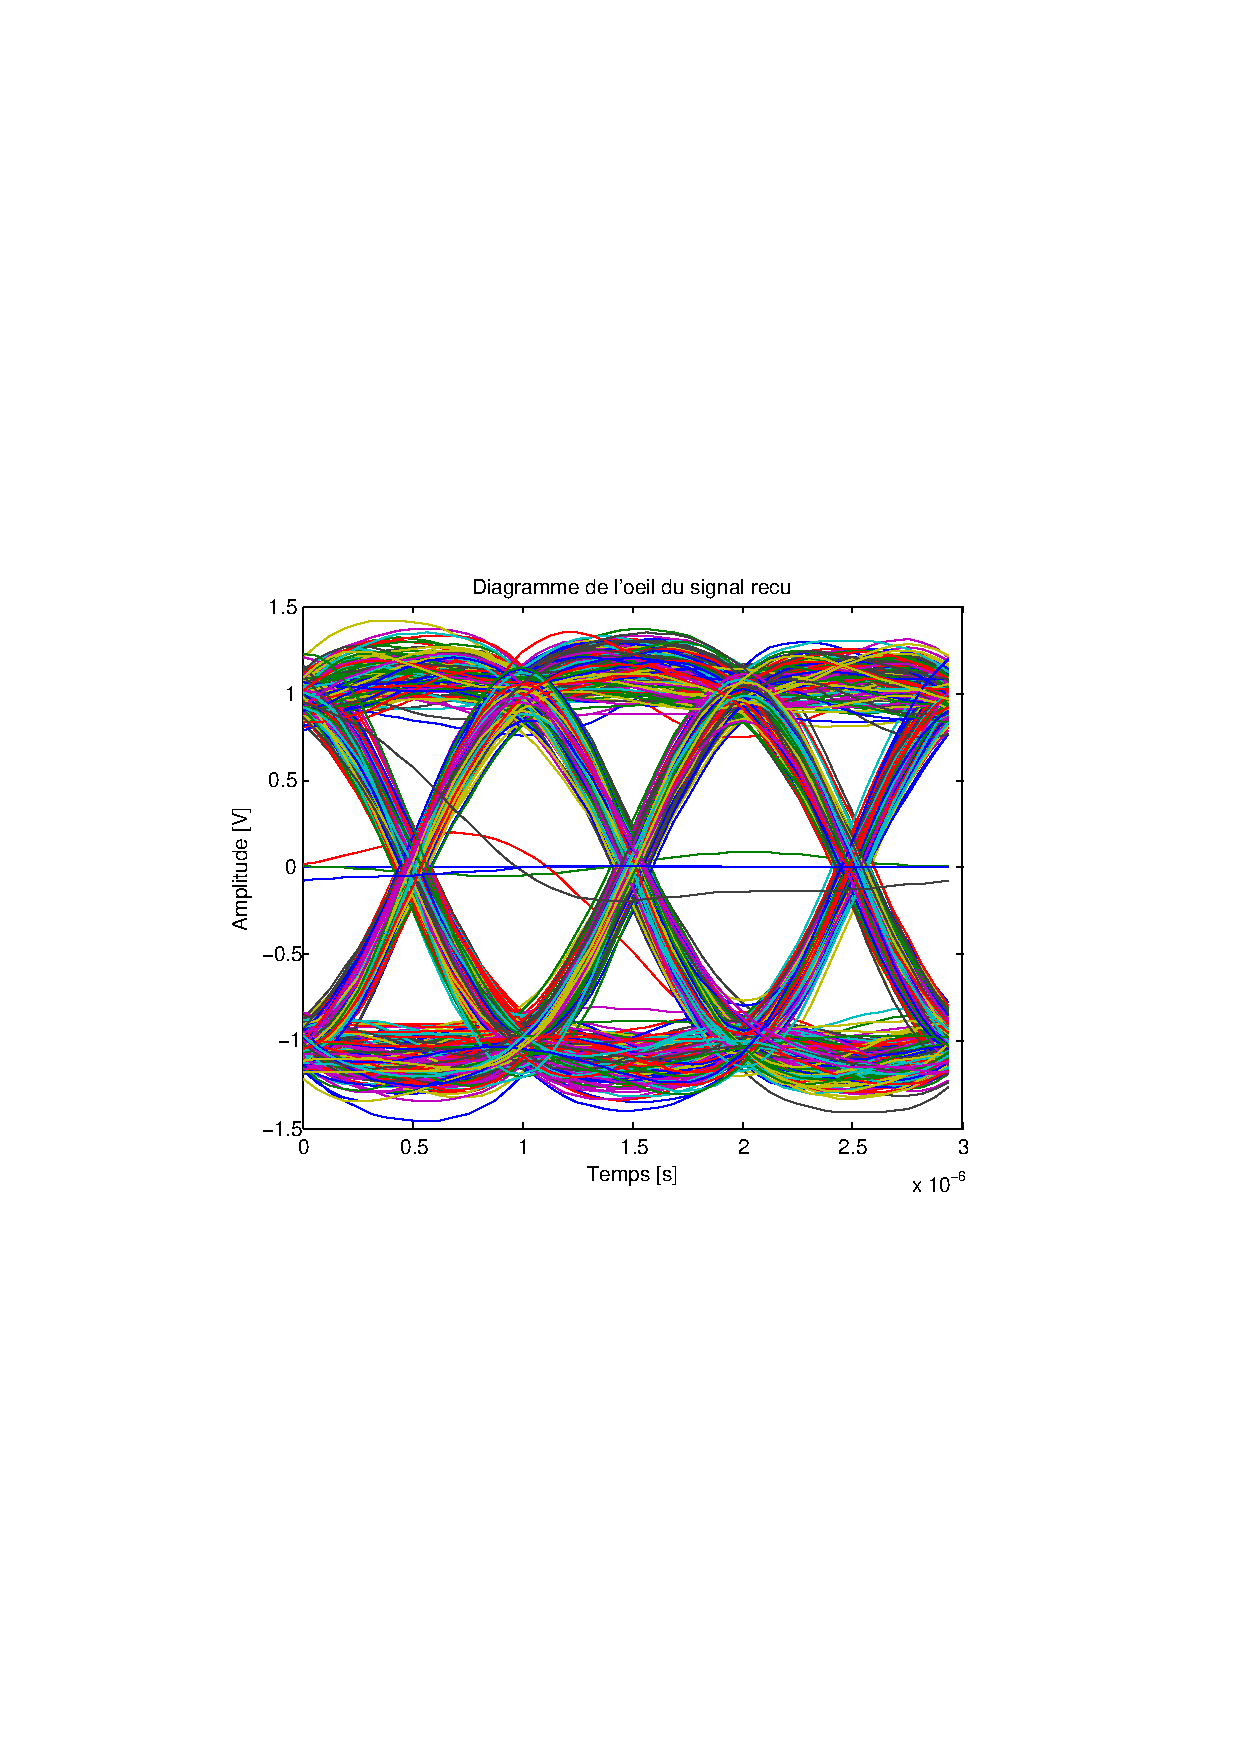
\includegraphics[width=1\linewidth]{Q10-alfa075.pdf}
  		\caption{Diagramme de l'oeil pour $\alpha$ = 0.75}
  		\label{fig:q10a075}
	\end{subfigure}
	\caption{Différentes diagrammes de l'oeil à différentes $\alpha$.}
	\label{fig:q10a}
\end{figure} 

\begin{figure}
	\begin{subfigure}{.5\textwidth}
  		\centering
  		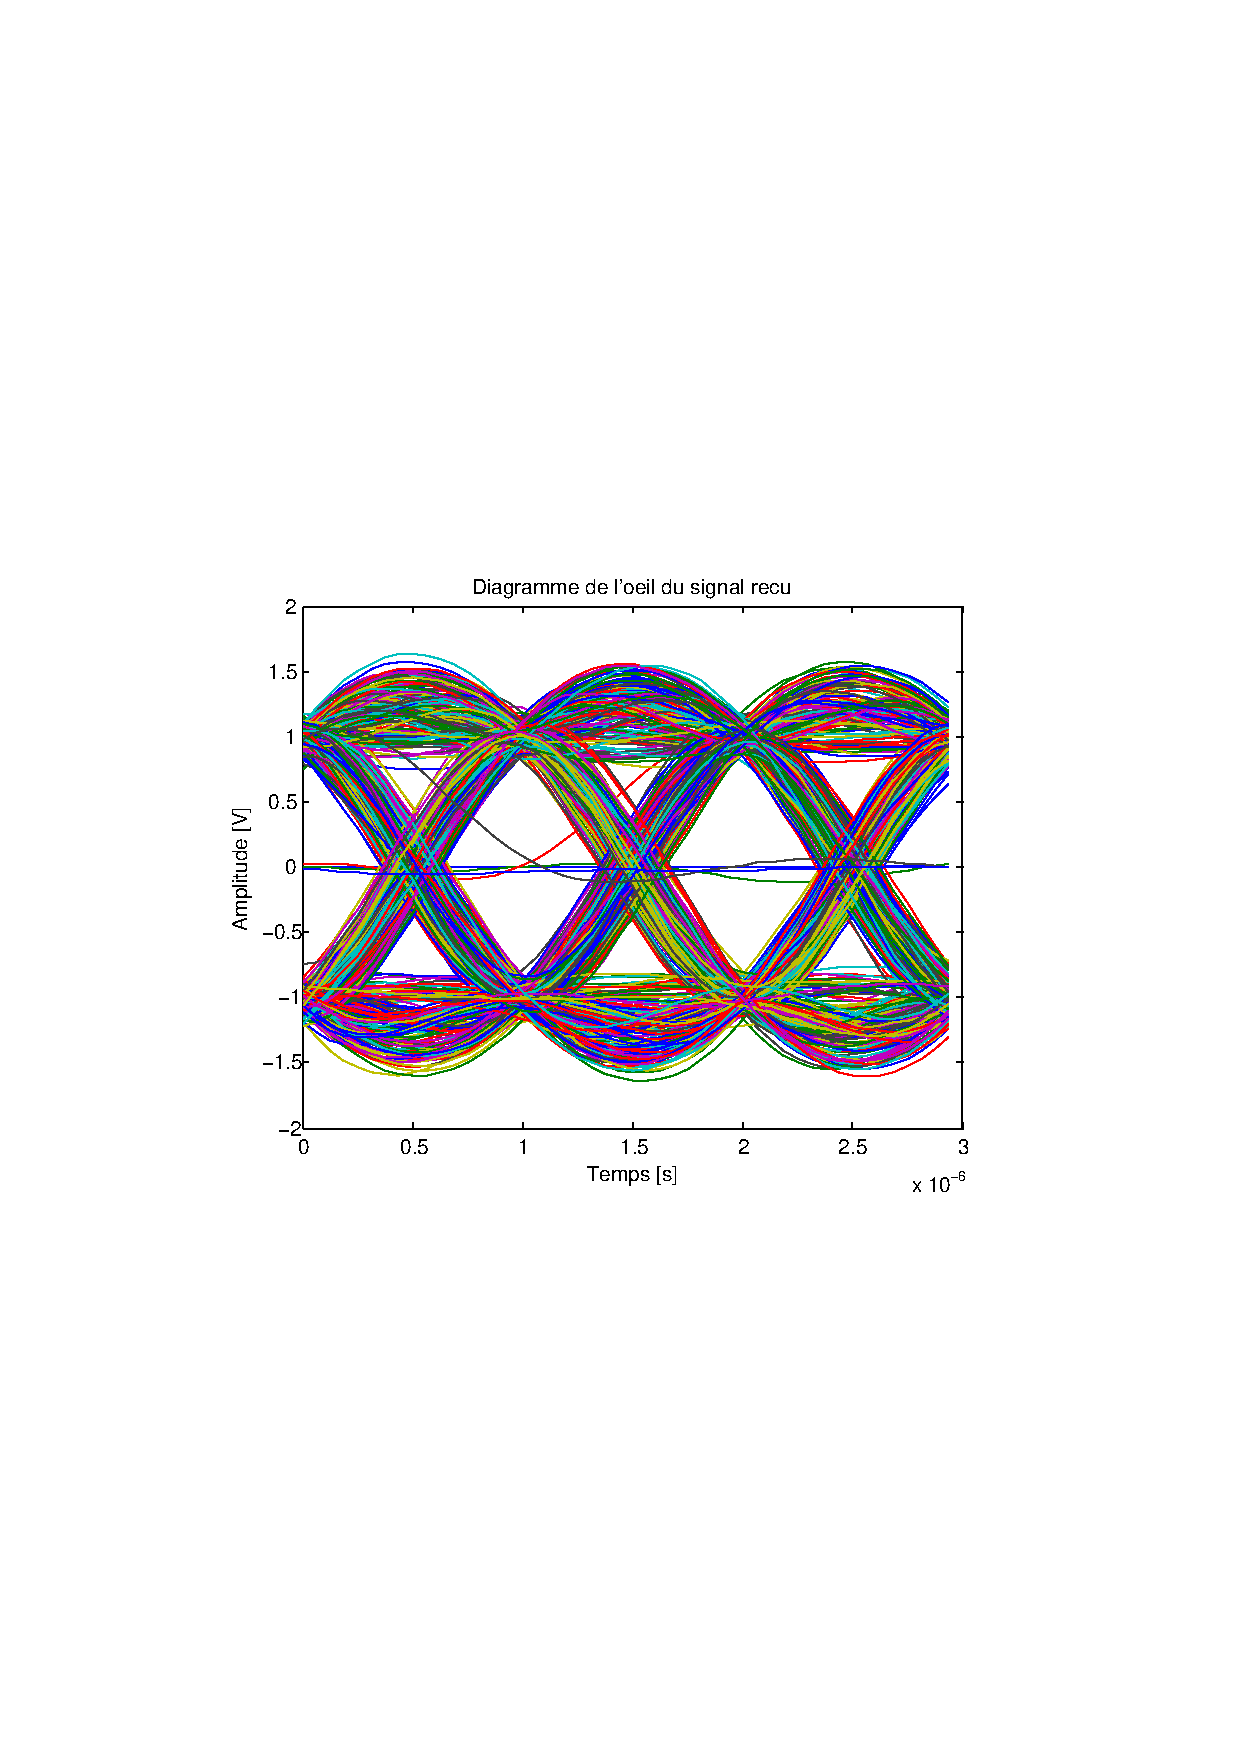
\includegraphics[width=1\linewidth]{Q10-EbNo20.pdf}
  		\caption{Diagramme de l'oeil pour L = 8}
  		\label{fig:q10l16}
	\end{subfigure}
	\begin{subfigure}{.5\textwidth}
  		\centering
  		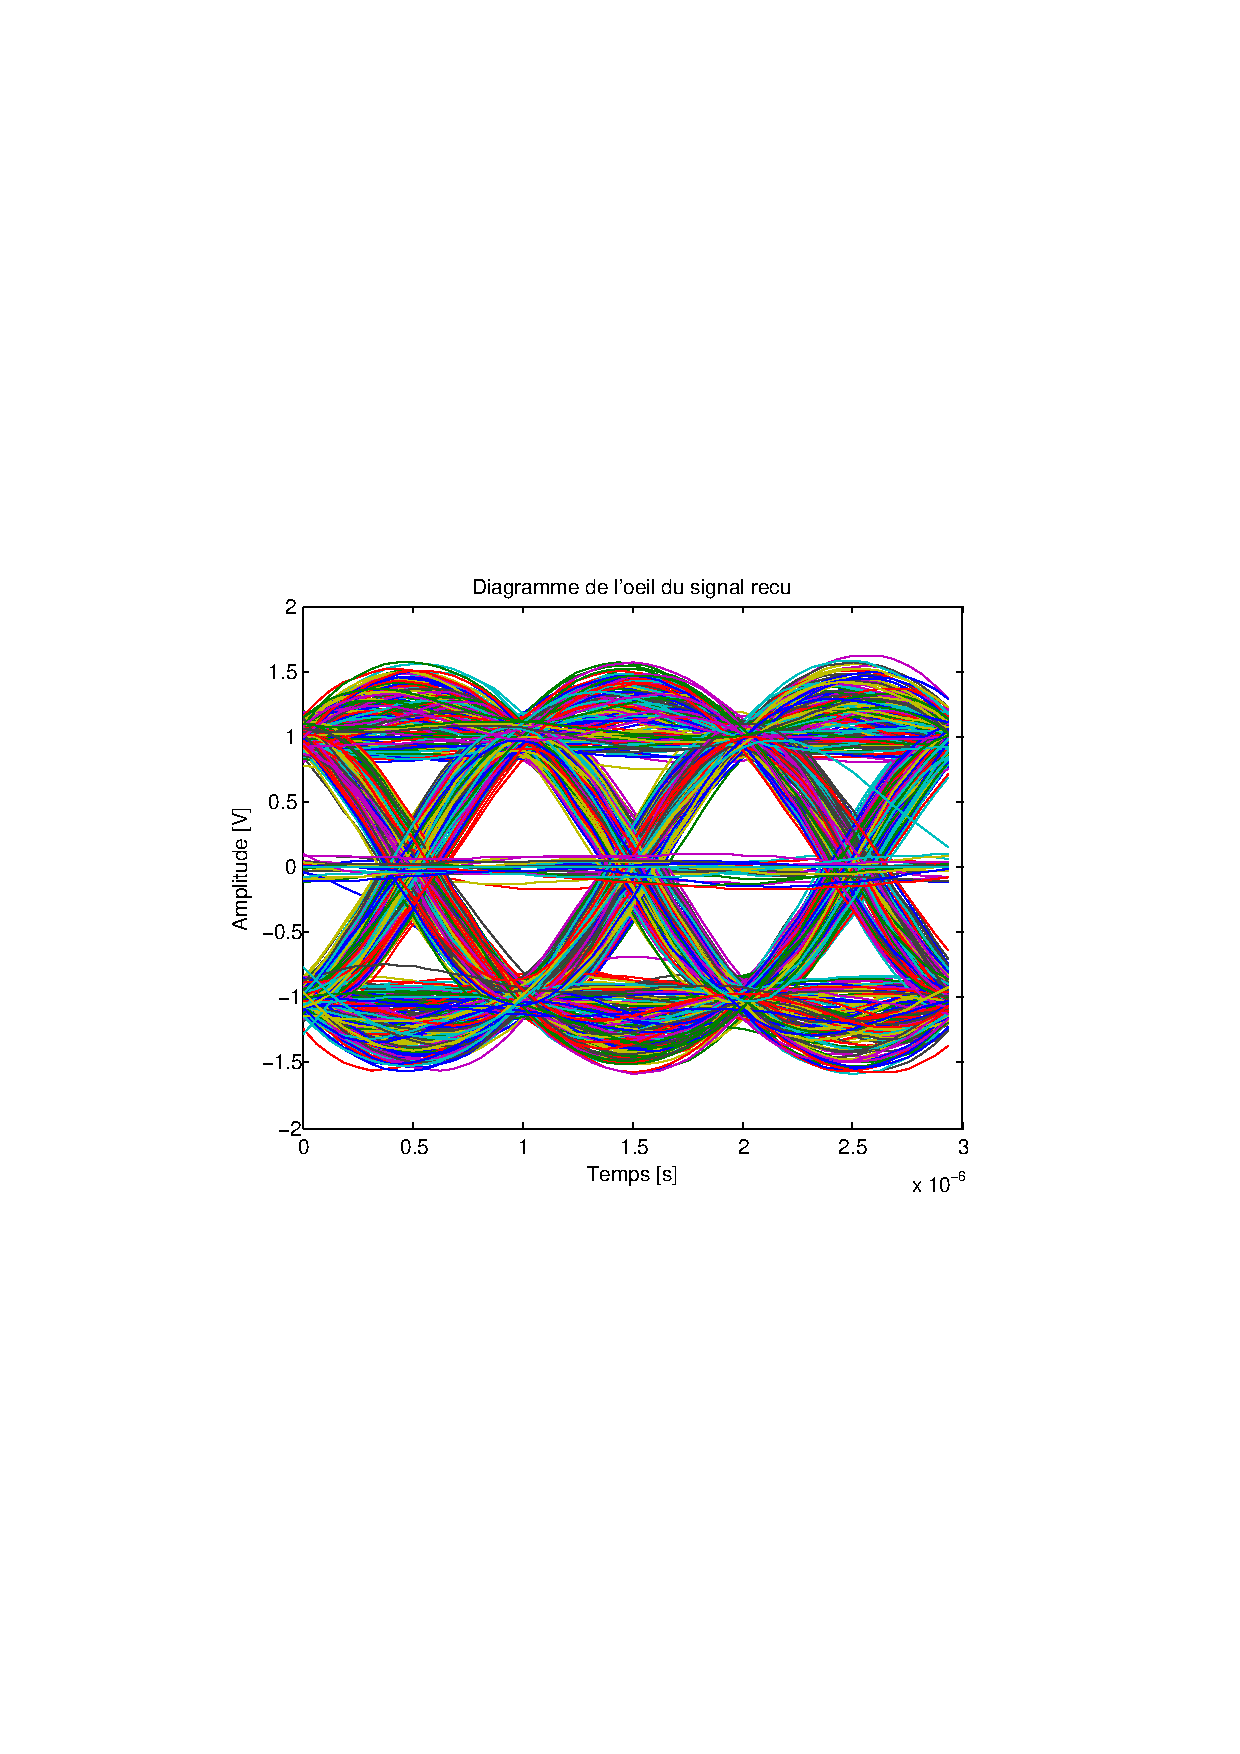
\includegraphics[width=1\linewidth]{Q10-L64.pdf}
  		\caption{Diagramme de l'oeil pour L = 64}
  		\label{fig:q10l64}
	\end{subfigure}
	\caption{Différentes diagrammes de l'oeil à différentes valeurs de L.}
	\label{fig:q10l}
\end{figure} 
\begin{figure}
	\begin{subfigure}{.5\textwidth}
  		\centering
  		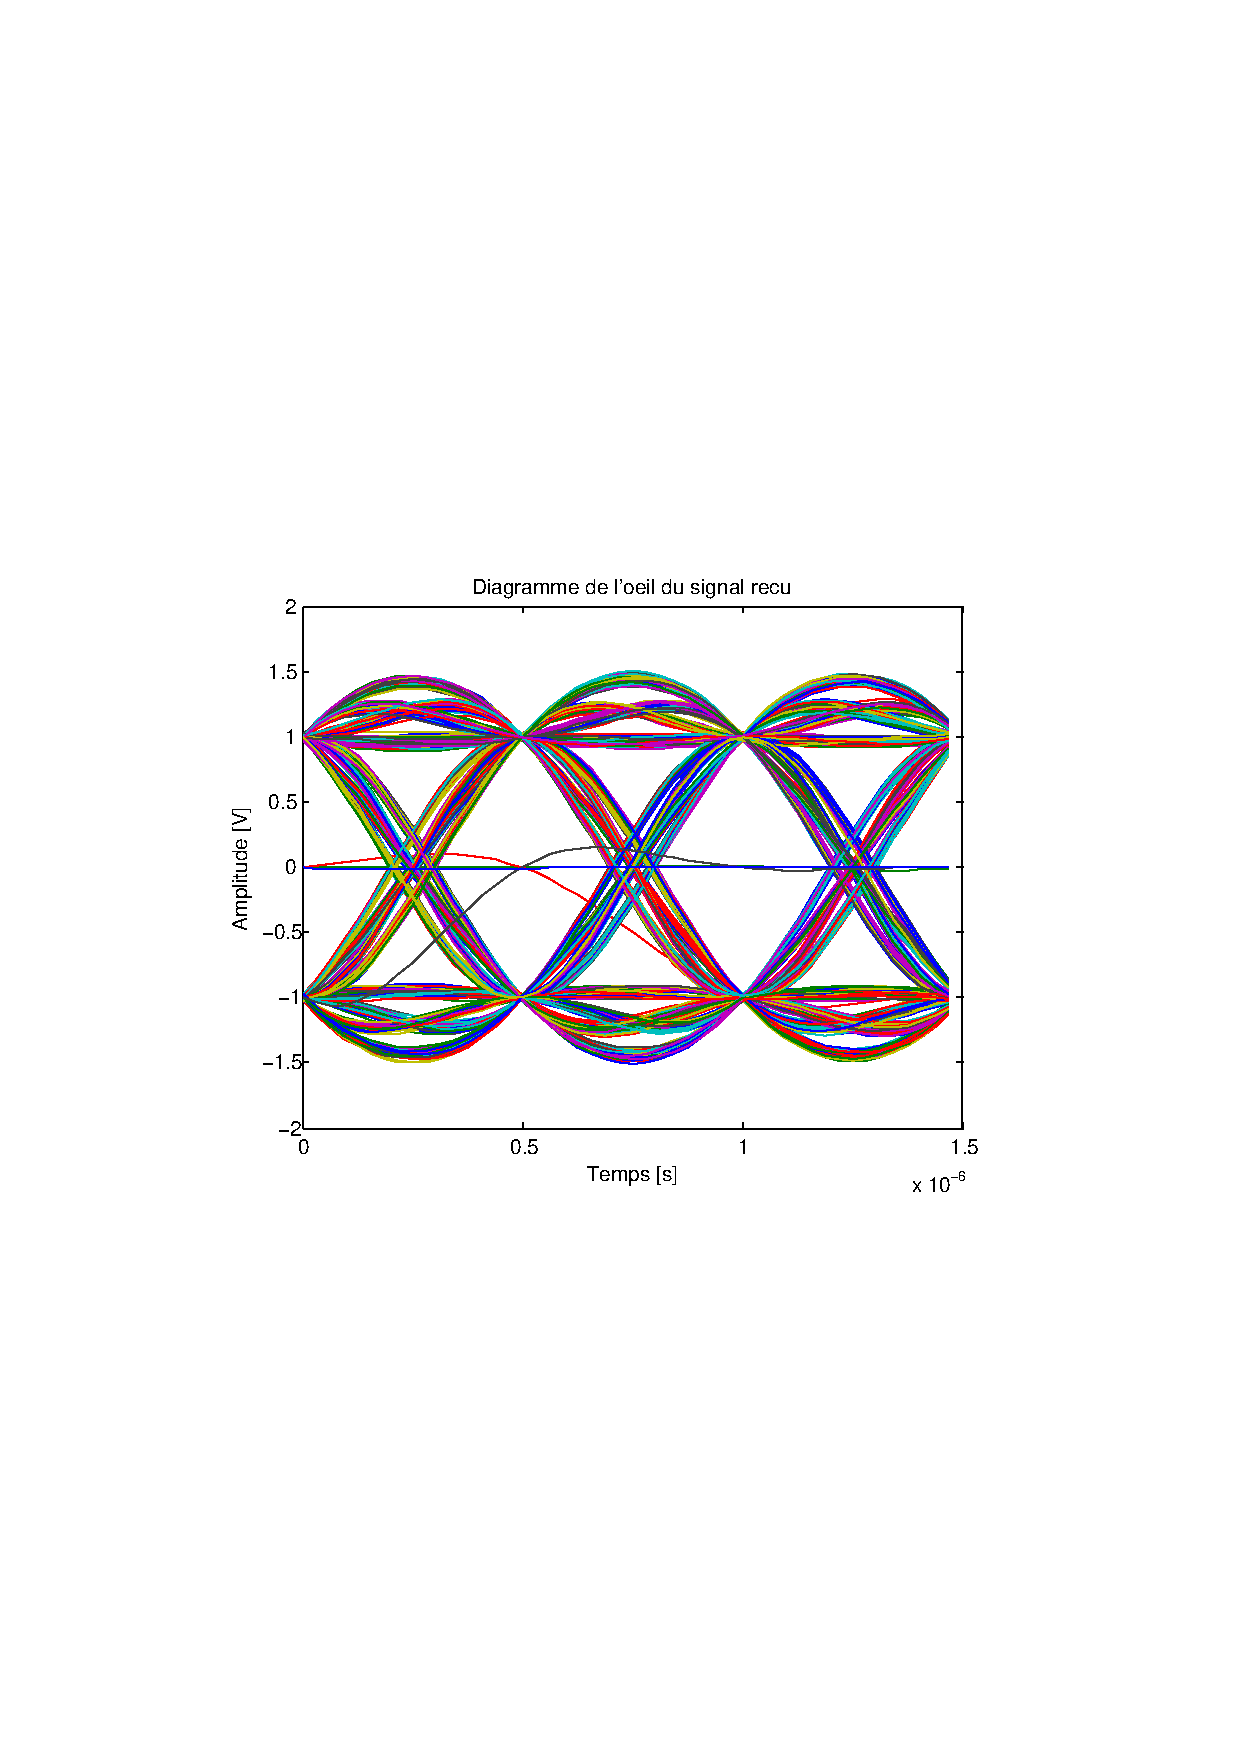
\includegraphics[width=1\linewidth]{Q10-Tsur2.pdf}
  		\caption{Diagramme de l'oeil pour T = $\frac{1}{2*D}$}
  		\label{fig:q10t2}
	\end{subfigure}
	\begin{subfigure}{.5\textwidth}
  		\centering
  		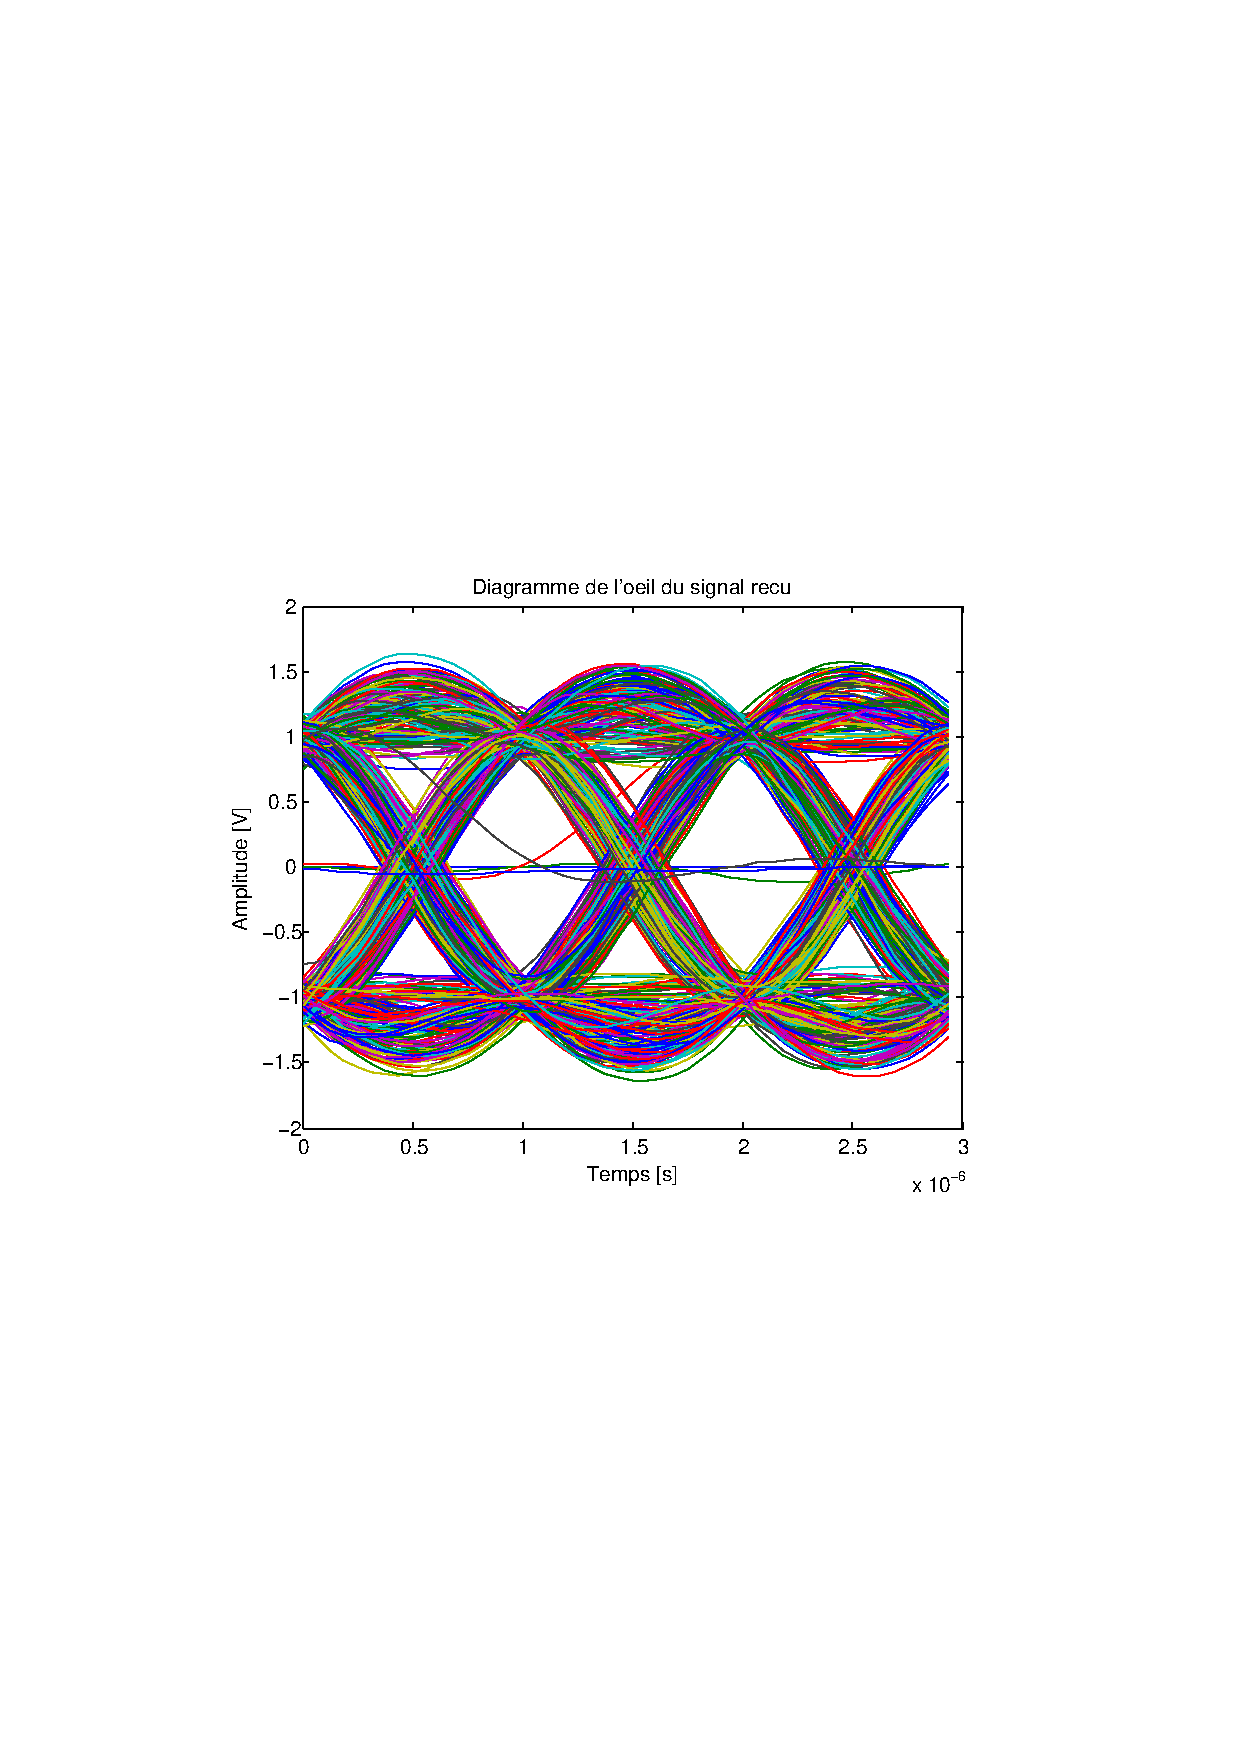
\includegraphics[width=1\linewidth]{Q10-EbNo20.pdf}
  		\caption{Diagramme de l'oeil pour T = $\frac{1}{D}$}
  		\label{fig:q10t1}
	\end{subfigure}
	\caption{Différentes diagrammes de l'oeil à différentes $\alpha$.}
	\label{fig:q10t}
\end{figure} 



\subsection{Décimation}
\subsubsection*{Question 11}
Après le filtre adapté il faut prendre les valeurs $y_k$ qui conviennent. Comme c'était mentionné au-dessus le but du filtre adapté c'est de maximiser le \emph{RSB}, donc c'est pour cela qu'en ayant deux signaux de la même longueur, alors le résultat maximum de la convolution se trouvera à la valeur de la longueur. Dans ce cas sera tous les \emph{LT}. 
\subsubsection*{Question 12}
C'est très important d'avoir de la synchronisation dans un système de transmission, car si ce n'est pas comme cela on échantillonnera le signal reçu dans le temps invalide et cela puisse arriver parce qu'un canal à \emph{BBG} ajoute aussi un déphasage au signal. Finalement, si c'est le cas, le filtre adapté ne maximisera pas le \emph{RSB} dans le temps de symbole.\section{Prise de décision \emph{(demapping)}}
\subsubsection*{Question 13}
Dans la suite de la chaîne de communication, une fois que les symboles $y_k$ sont reçus il faut prendre un seuil de décision. À l'aide la figure \ref{fig:q13} on voit que le seuil optimal est en \emph{0}. 
\begin{figure}
	\begin{center}
	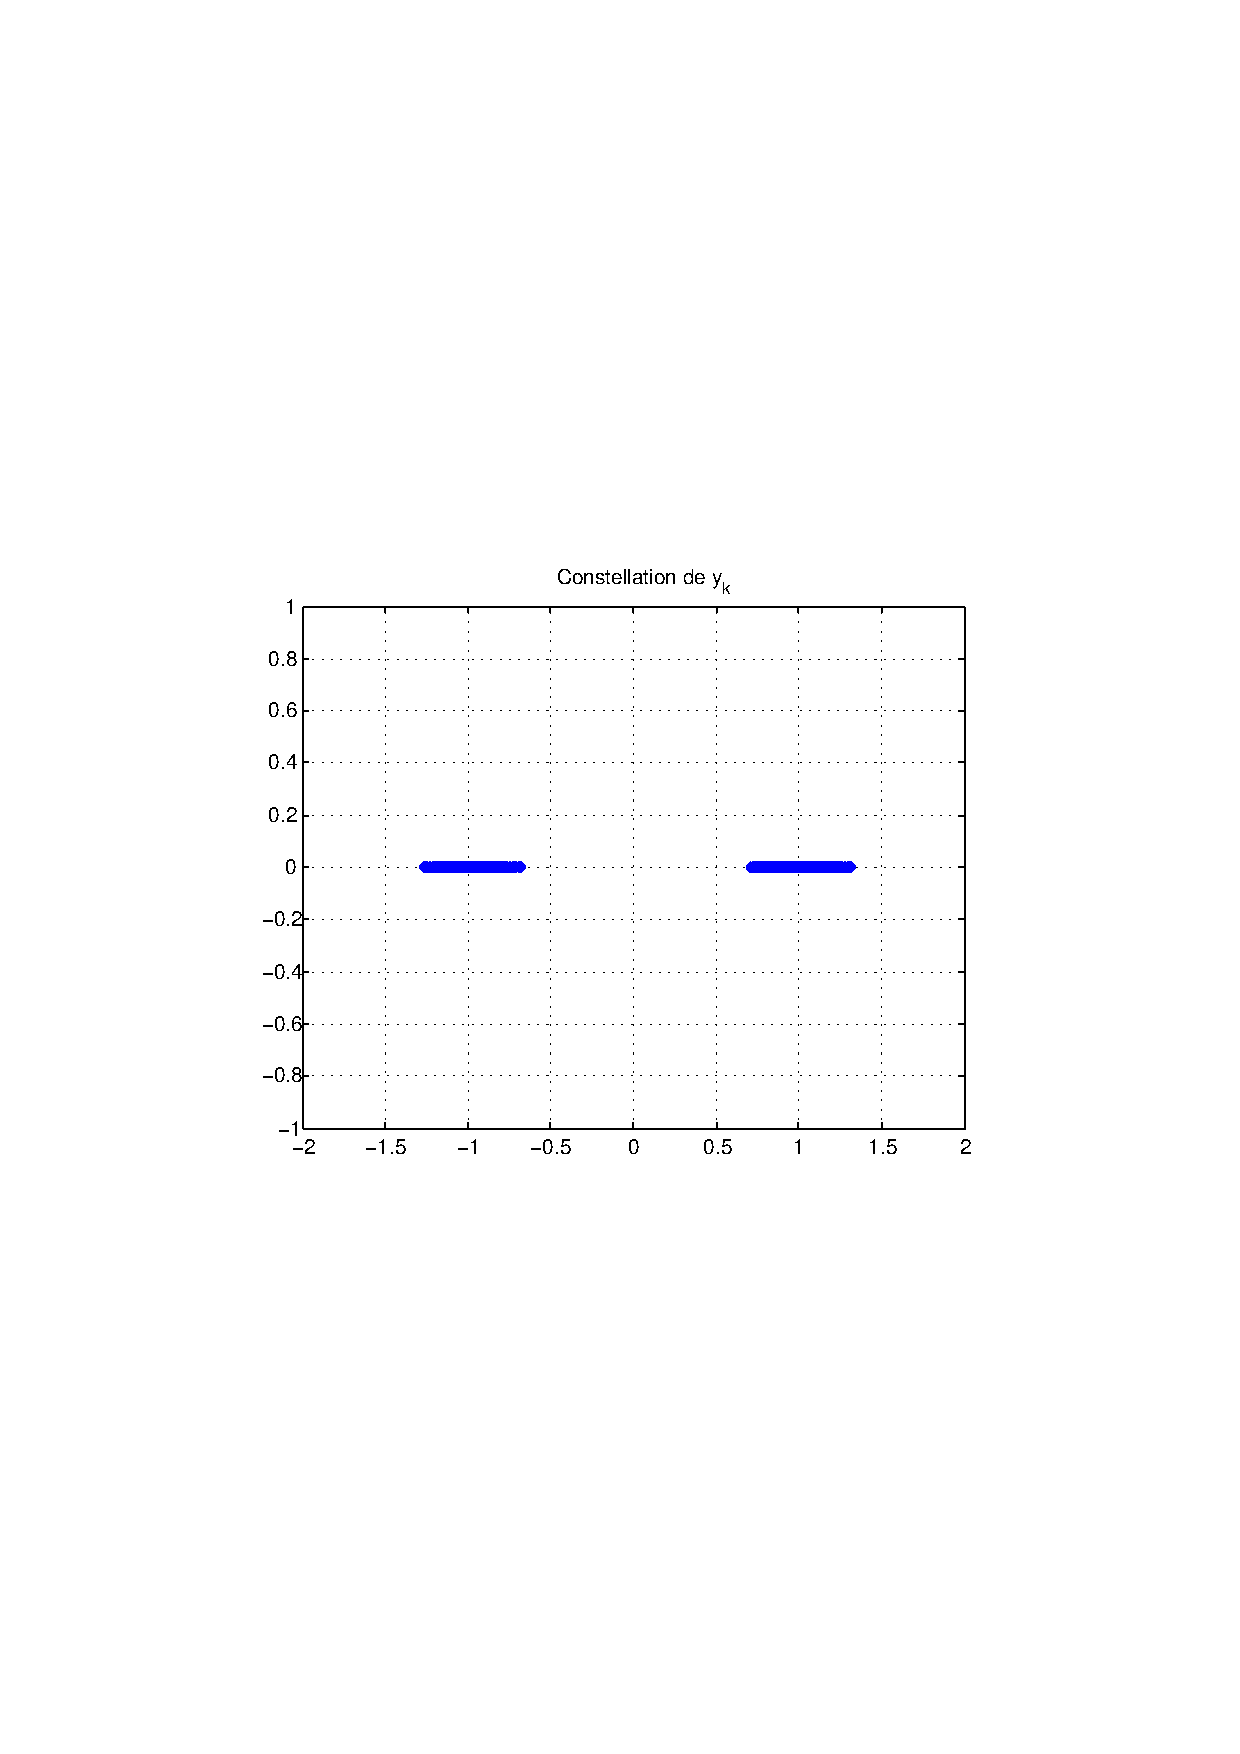
\includegraphics[scale=0.5]{Q13.pdf}
	\caption{Constellation des $y_k$.}
	\label{fig:q13}
	\end{center}
\end{figure}  

\section{Calcul du taux d'erreur binaire}
Après le seuil optimal il faut comparer et trouver combien d'erreurs on a commit dans la transmission des symboles. Donc c'est avec le \emph{TEB} dans lequel on calcule le rapport entre le nombre d'éléments binaires faux et le nombre d'éléments binaires transmis.
\section{Mesures de performances}
Finalement, c'est important mesurer la chaîne de transmission. C'est fait avec la relation entre le \emph{RSB} et la probabilité d'erreur.
\subsubsection*{Question 14}
Dans la figure \ref{fig:q14} on trouve les deux courbes de \emph{BER}. Ici la courbe empirique arrive qu'à 7dB de \emph{EbNo} car pour pouvoir continuer c'est neccesaire d'envoyer plus qu'un million de bits et étant donné les limitations de mémoire c'était impossible. L'important est que c'est évident que la courbe empirique est pire que la théorique, quelque chose qui est attendu, car la courbe théorique est fait à partir d'estimations et méthodes statistiques qui ne prennent pas certains aspects de la chaîne de transmission. Enfin, la courbe empirique doit être toujours pire que la théorique sauf quand on utilise des codes détecteurs et correcteurs d'erreurs ainsi que de la codification de canal.

\begin{figure}
	\begin{center}
	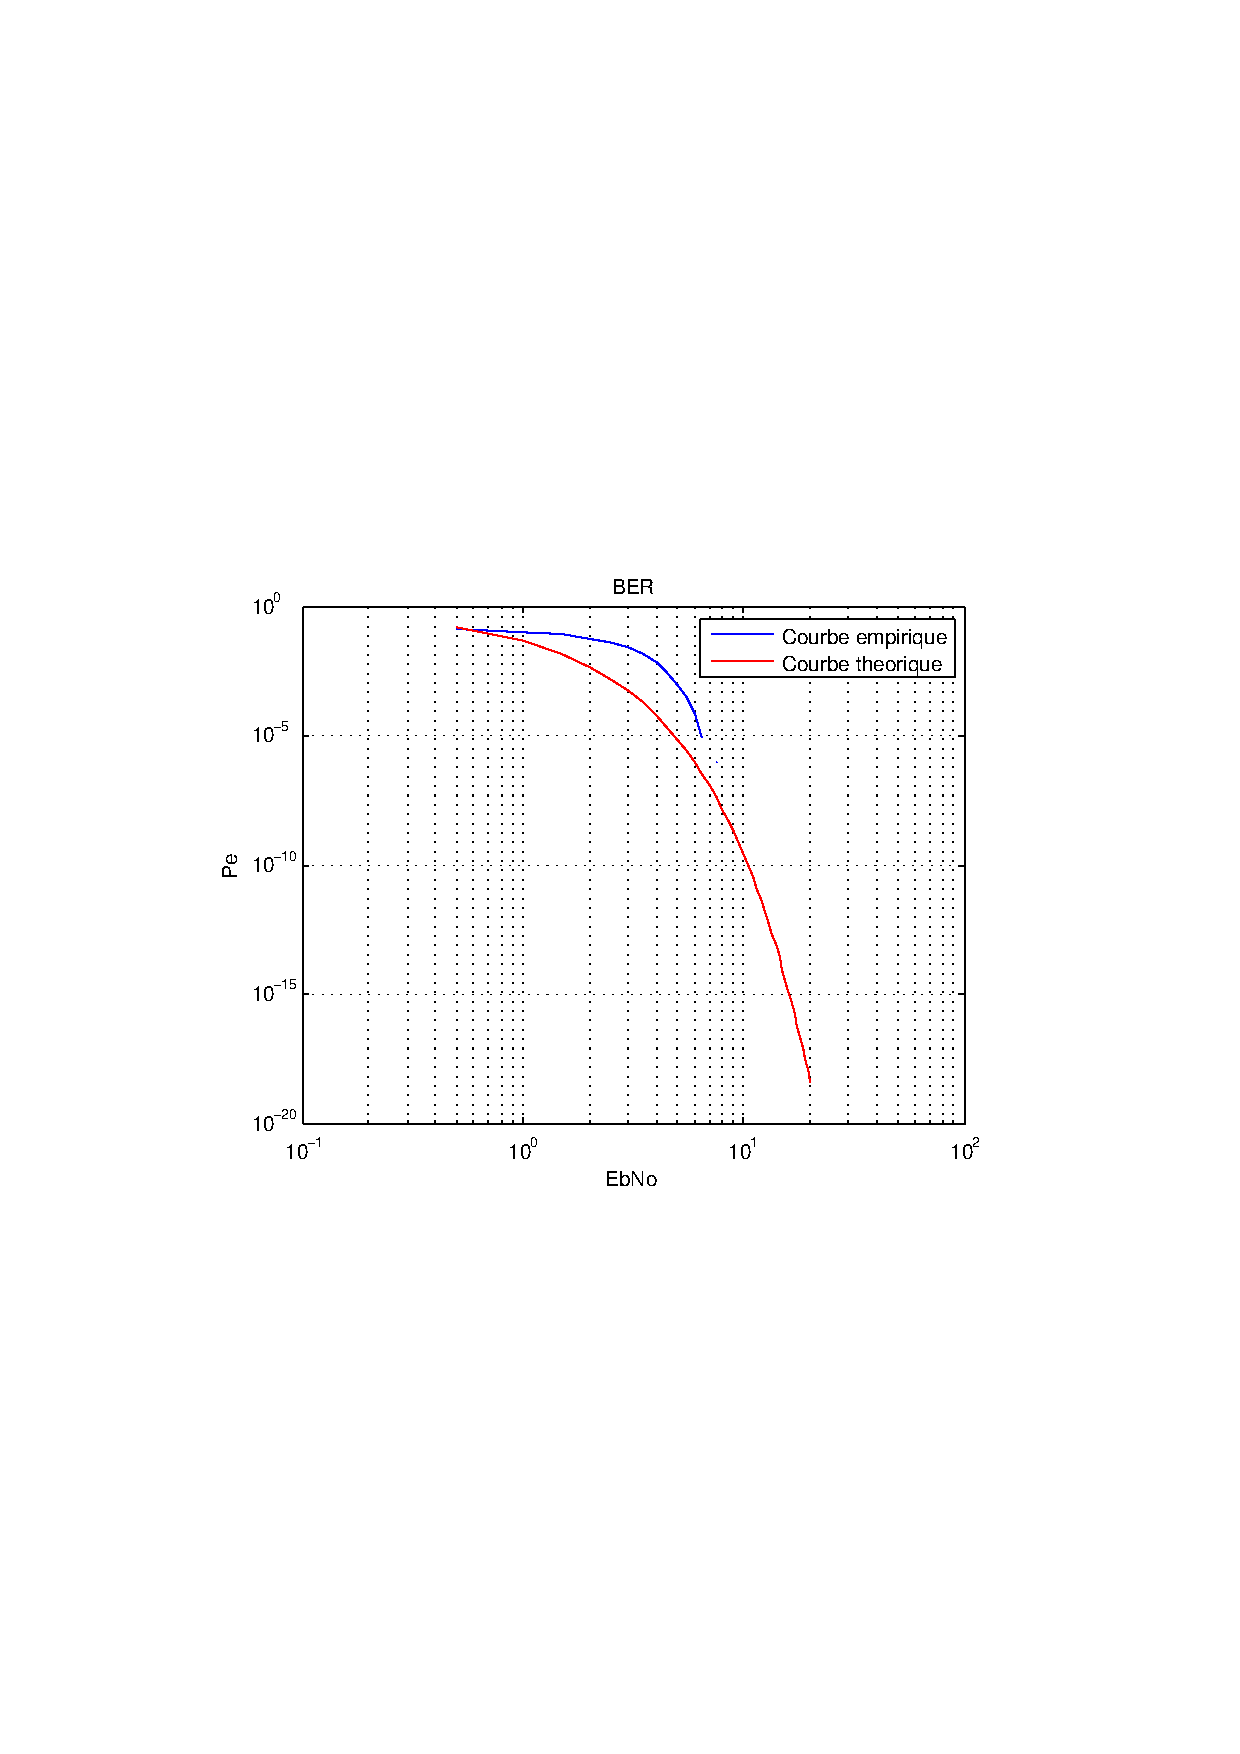
\includegraphics[scale=0.5]{Q14-BER.pdf}
	\caption{Constellation des $y_k$.}
	\label{fig:q14}
	\end{center}
\end{figure}  
%\begin{figure}[htb]
%\begin{center}
%\includegraphics[scale=0.5]{Q2total}
%\caption{TFD du signal complété par des zéros}
%\end{center}
%\end{figure}

\end{document}